\cotefile{43}
\scanpage{94}
Soit $\mathcal T'_k$ l'\unsure{espace} de Weil suivant : les objets sont les
\deleted{\unsure{quasi} \unsure{groupes} \unsure{quasi-algébriques}}
\deleted{\unsure{schémas}}
\unsure{quasi-schémas} \unsure{flasques} compacts, \unsure{la descente}
est donnée par les morphismes \deleted{\unsure{surjectifs}} \uuline{finis}
surjectifs. Soit $C'(k)$ la catégorie des faisceaux de Weil sur $\mathcal T'_k$.

\margin{Le \unsure{choix|désir} de ``fini'' est imposé par le désir d'avoir
une ``application continue'' $\mathcal T'_k\unsure{\longrightarrow|-}\mathcal T_S$ !}
\figure{\begin{tikzpicture}[x=1cm,y=1cm]
\draw(0,4.5)..controls(.9,5.1)and(.7,3.7)..(.9,3.1)..controls(1.4,1.1)and(.7,.8)..(-.1,0);
\end{tikzpicture}}

On a dans $C'(k)$ les foncteurs $H^i(k,G)$,
$\operatorname{Ext}^i(k;F,G)$, \inserted{$\underline{\operatorname{Ext}}^i_k(F,G)$}
et les relations habituelles
\[
\left\{\begin{aligned}
 H^i(k,F)&\simeq\operatorname{Ext}^i(k;\mathbb Z_k,F)\\
 \operatorname{Ext}^{\unsure{n|p+q}}(k;F,G)&\Longleftarrow
 H^p(k,\underline{\operatorname{Ext}}^{\unsure{q}}_k(F,G))
\end{aligned}\right.
\]

On notera que si $k$ est alg. clos, alors
$H^i(k,F)=0$ pour $i>0$. La formation des
$\underline{\operatorname{Ext}}^i_k(F,G)$ commute \unsure{à}
l'extension du corps de base\unsure{\ldots}

Il y a lieu de \deleted{\unsure{calculer}} donner des règles de calcul
pour des $H^i(k,G)$, $\operatorname{Ext}^i(k;F,G)$ si $G$ provient d'un
\inserted{quasi-}\unsure{schéma} en groupes habituel sur $k$,
[p.ex. d'un \unsure{pro.gr.} de Serre de type ``spécial'', i.e. à
morphismes de transition \unsure{affines|finis} pour l'indice grand\unsure{\ldots}].
Il faudrait prouver alors que ($k$ est parfait)

\noindent a) si $G$ est \unsure{simple} sur $k$, les $H^i(k,G)$ sont les
$H^i(k,\widetilde G)$, où $\widetilde G$ est le faisceau de Weil associé\ldots

\noindent b) Kif-kif pour les $\operatorname{Ext}^i(k;F,G)$\ldots
\mspage{93}

\scanpage{95}
Il faudrait aussi, de façon générale (dans le contexte ``quasi'') étudier
\deleted{\unsure{le}} si $H^i(k,G)$ peut se calculer comme une cohomologie
galoisienne\ldots
\margin{\figure{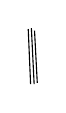
\begin{tikzpicture}[x=1cm,y=1cm]
\draw (0,0)--(-.03,.7); \draw (.045,0)--(.01,.71); \draw (.085,.015)--(.05,.68);
\end{tikzpicture}}}

\deleted{N.B. Il n'y \unsure{a pas} \illegible{3} \unsure{élémentaire} de
Weil \unsure{permette}.}
\mspage{94}

\scanpage{96}
On va définir un foncteur fondamental \inserted{dit \uline{de Néron}}
\[
\mathcal N:C(S)\longrightarrow C'(k).
\]
Pour ceci, si $F$ est un faisceau de Weil sur $S$, on définit un faisceau
de Weil sur $\mathcal T_k$ en prenant, pour tt anneau \unsure{comm.} $A$ sur $k$
\inserted{\[
\simeq F(\varinjlim_{P}\mathbb V(A^P))
=F(\varprojlim_{P}\operatorname{Spec}(\mathbb V(A^P)))
\qquad\inserted{\operatorname{Spec}(\varinjlim_{P}\mathbb V(A^P))}
\]}
\[
\begin{aligned}
\mathcal N(F)(A)&=\varinjlim_{P}
 F\left(\unsure{\operatorname{Spec}}\left(\mathbb V
 \left(\underbrace{\prod_{i\in I_P} A_i^P}_{A^P}\right)\right)\right)\\
 &=\underline{\lim}_{P}\prod_{i\in I_P}F(\mathbb V(A_i^P)).
\end{aligned}
\]
\margin{N.B. On a en fait une ``application continue''
$\mathcal T'_k\longrightarrow\mathcal T_S$, \unsure{correspondant}
aux \unsure{pro-objets}, d'où le foncteur image directe de faisceaux, et
ses propriétés ``formelles''\ldots ! ? !}
\figure{\begin{tikzpicture}[x=1cm,y=1cm]
\draw(0,5)..controls(1.4,6.5)and(1.6,5)..(2.2,4.5)..controls(3,3.3)and(1,1)..(-.2,0);
\end{tikzpicture}}

$P$ parcourt les ``partitions constructibles finies'' de $A$, et où pour
une telle $P$, $I_P$ est son ensemble d'indices, et $A_i^P$ les composantes
correspondantes de $A$. En d'autres termes, un \unsure{quasi-schéma}
\unsure{flasque} \inserted{cpt} étant considéré comme un pro-(schéma affine)
sur $k$, on le transforme par $\mathbb V$ en un pro (schéma affine) sur $S$,
et on lui applique le foncteur $F$.
\deleted{[N.B. $\mathcal N(F)$ est compatible \unsure{avec} les limites
inductives d'anneaux \unsure{donc si on y tient}, on peut se limiter}
\margin{Non, car le foncteur $\mathbb V:k\text{-alg}\longrightarrow V\text{-alg.}$
ne commute pas aux limites inductives\ldots}
\mspage{95}

\scanpage{97}
\deleted{dans la catégorie $C'(k)$ aux foncteurs compatibles avec les
limites inductives.}

On constate que le foncteur $\mathcal N$ qu'on vient de définir est exact
à gauche, \unsure{et} transforme groupes comm. en groupes comm., d'où
$C(S)\longrightarrow C'(k)$. On pose aussi
\[
\mathcal N(F)=\underline H^0_{S/k}(F)
\]
et \deleted{\unsure{de}} par suite
\[
R^i\mathcal N(F)=\underline H^i_{S/k}(F).
\]
Notons l'isomorphisme
\[
H^0_S\simeq H^0_k\circ\underline H^0_{S/k}
\]
et d'autre part que $\underline H^0_{S/k}$ \uline{transforme injectifs en injectifs}
\margin{à vérifier\ldots}
\deleted{\unsure{car on va voir} en construisant un adjoint à
$\mathcal N=\underline H^0_{S/k}$ et constatant que ce dernier est exact
à gauche :
\[
\operatorname{Hom}(\Phi,\mathcal N(F))\simeq
\operatorname{Hom}(\mathcal N^*(\Phi),F).
\]}
D'où une suite spectrale de Leray
\[
H^*(S,F)\Longleftarrow H^p(k,\underline H^q_{S/k}(F)).
\]
\mspage{96}

\scanpage{98}
Plus généralement, définissons
\[
\underline{\operatorname{Hom}}_{S/k}(F,G)=
\underline H^0_{S/k}(\underline{\operatorname{Hom}}_S(\unsure{F|G},G))
\]
\deleted{\unsure{Alors}} et \inserted{notons} les foncteurs dérivés de
$G\longmapsto\underline{\operatorname{Hom}}_{S/k}(F,G)$ par
\[
\underline{\operatorname{Ext}}^i_{S/k}(F,G).
\]
On a alors, si on admet que pour $G$ injectif,
$\underline{\operatorname{Hom}}_S(F,G)$ est acyclique pour
$\underline H^0_{S/k}$, \deleted{et pour $H^0_S$}, les suites spectrales
\margin{vérifier\figure{\begin{tikzpicture}\draw(0,0)--(0,1.1);\end{tikzpicture}}}
\[
\underline{\operatorname{Ext}}^{*\deleted{\unsure{p+q}}}_{S/k}(F,G)
\Longleftarrow\underline H^p_{S/k}
(\underline{\operatorname{Ext}}^q_S(\unsure{F|k},G))
\]
et compte tenu de
\[
\operatorname{Hom}_S(F,G)\simeq
H^0(k,\underline{\operatorname{Hom}}_{S/k}(F,G))
\]
et admettant que pour $G$ injectif,
$\underline{\operatorname{Hom}}_{S/k}(F,G)$ est acyclique pour $H^0(k,-)$,
on trouve
\margin{vérifier\figure{\begin{tikzpicture}\draw(0,0)--(0,1.1);\end{tikzpicture}}}
\[
\operatorname{Ext}^*(S;F,G)\Longleftarrow
H^p(k,\underline{\operatorname{Ext}}^q_{S/k}(F,G)).
\]
Enfin on aura
\[
\underline H^*_{S/k}(F)\simeq
\underline{\operatorname{Ext}}^*_{S/k}(\mathbb Z_S,F).
\]

Notations et remarques analogues en partant de faisceaux sur
$U\unsure{\subset|\in}S$, au lieu de $S$.
\mspage{97}

\scanpage{100}
\margin{$S\unsure{\sigma|\gamma}=(D\Delta\unsure{\sigma|\gamma}_K)(1)$}
\figure{\begin{tikzpicture}[x=1cm,y=1cm]
\draw[->](.7,0)..controls(-.6,0)and(-.5,.2)..(-.4,.7)..controls(-.4,1.1)and(.5,1.3)..(.8,1.6)..controls(1,1.9)and(.7,2.2)..(.3,2.6)..controls(-.1,3)and(.9,3.1)..(1.6,3.4);
\end{tikzpicture}}
\[
\underset{\sim}{\operatorname{Ext}}^i_{K/k}(G,S\underline{\unsure{\sigma|\gamma}})
\xrightarrow{\sim}
\underset{\sim}{\operatorname{Ext}}^{i\unsure{*}}_{k\text{-gr}}
(\Gamma^{\deleted{\unsure{*}}}G^*,\unsure{\sigma|\gamma})
\]
isom si $G$ \uline{affine} sans \unsure{composantes} $G_a$
\[
\underset{\sim}{\underline{\operatorname{Ext}}}^{i}_{K/k}(G,S\unsure{\sigma|\gamma})
\longrightarrow
\underset{\sim}{\underline{\operatorname{Ext}}}^{2i}(\Gamma G^*,\unsure{\sigma|\gamma})
\]
pour
\[
\underline{\operatorname{Ext}}^i_{K/k}(G,S\unsure{\sigma|\gamma})
\longrightarrow \underline{\operatorname{Ext}}^i
\]
\margin{\deleted{$\unsure{\Gamma}_{K/k}G$}\quad $R^*f_{K/k}$}

\noindent 1) $K$-\uline{groupes algébriques}.
\diagram{\begin{tikzcd}[column sep=large,row sep=small]
 & \text{nul pr }i>2\arrow[d,dash,bend right] & \\
\operatorname{Ext}\arrow[d,dash] &
\underline{\operatorname{Ext}}\arrow[d] & H^p\arrow[d]\\
\begin{gathered}\text{nature arithmétique}\\\text{ie ``globale''}\end{gathered} &
\begin{gathered}\text{nature}\\\text{géom.}\end{gathered} &
\begin{gathered}\text{nature arithmétique}\\\text{ie. ``globale''}\end{gathered}
\end{tikzcd}}
\uline{de $K$-groupes algébriques}

\noindent 2) \uline{Dualité de Cartier}. Extension aux
$\unsure{\mathcal K|\mathcal R}\operatorname{Gr}_K$

\margin{\figure{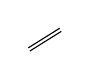
\begin{tikzpicture}\draw (0,0)--(.4,.25);\draw (.02,-.04)--(.42,.21);\end{tikzpicture}}}
\noindent 3) \unsure{Quasi-groupes} algébriques, leurs
$\operatorname{Ext},\underline{\operatorname{Ext}},H^p$

\noindent 4) \uline{Dualité de Serre-\unsure{Pontrjagin}}

\noindent 5) Le foncteur $\underline\Gamma_{K/k}$
\inserted{de Néron-\unsure{Weil}}

\margin{\figure{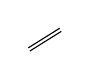
\begin{tikzpicture}\draw (0,0)--(.4,.25);\draw (.02,-.04)--(.42,.21);\end{tikzpicture}}}
\noindent 6) Les foncteurs \deleted{$\unsure{\Gamma}_{K/k}$}
\[
\underset{\sim}{\underline{\operatorname{Ext}}}^{*}_{K/k}(F,G),
\quad\underset{\sim}{\underline H}^{*}_{K/k}(G)
\]
\inserted{\[
E^*_{K/k}(F,G)\qquad E_{K/k}(G)
\]}
\margin{nul pr $i>3$}

\noindent 7) L'hom. fondamental.

\margin{\figure{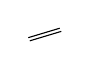
\begin{tikzpicture}\draw (0,0)--(.4,.12);\draw (.02,-.04)--(.42,.08);\end{tikzpicture}}}
\noindent 8) Le th. de dualité.
\mspage{99}

\scanpage{101}
\mspage{100}
\mspage{22.}
proves one half of (6.5) in all cases.

The problem of determining the actual numbers $q_k$ in (6.5) is thus
seen to be a special case of the more general problem of determining
the structure of the group $J(X)$. An attack on this problem by the
methods of [2] and [3] will be given in a future publication.

We conclude with a few remarks on the relation between the methods of
this paper and those of James. The main tool of James is the ``intrinsic
join''. Actually he defines several ``intrinsic joins'', two of them
being maps
\[
\begin{aligned}
Q_{n,k}*P_{m,k}&\longrightarrow P_{m+n,k}\\
Q_{n,k}*Q_{m,k}&\longrightarrow Q_{m+n,k},
\end{aligned}
\]
where $X*Y$ denotes the join of $X$ and $Y$. Since
$X*Y=S(X\mathbin{\times\mkern-10mu\times}Y)$\inserted{${}^+$}
these two maps can, in view of (2.4) (4.3) and (5.4), be written
\[
\begin{aligned}
P_k^{(n-k)\xi\oplus\eta}\mathbin{\times\mkern-10mu\times}
P_k^{(m-k)\xi}&\longrightarrow P_k^{(m+n-k)\xi}\\
P_k^{(n-k)\xi\oplus\eta}\mathbin{\times\mkern-10mu\times}
P_k^{(m-k)\xi\unsure{\oplus\eta}}&\longrightarrow
P_k^{(m+n-k)\xi\oplus\unsure{\zeta|\eta}}.
\end{aligned}
\]
In view of (4.5) both these are maps of the type
\[
f:X^\alpha\mathbin{\times\mkern-10mu\times}X^\beta
\longrightarrow X^{\alpha+\beta+\tau}
\]
where $X$ is a compact differentiable manifold with tangent bundle
$\tau$. By (3.3), and the fact that the smash product commutes with
duality, the dual of $f$ is a map of the form:
\[
Df:X^{\gamma+\delta}\longrightarrow
X^\gamma\mathbin{\times\mkern-10mu\times}X^\delta
\]
where $\gamma=-\alpha-\tau$, $\delta=-\beta-\tau$. Now the diagonal map
$X\longrightarrow X\times X$ induces a map
\[
\Delta:X^{\gamma+\delta}\longrightarrow(X\times X)^{\gamma\times\delta}
=X^\gamma\mathbin{\times\mkern-10mu\times}X^\delta
\quad\text{by (2.3).}
\]
It would seem reasonable to suppose that the maps $Df$ and $\Delta$ are
of the same $S$-homotopy type.

In addition to the maps first mentioned James also defines an intrinsic
join for the Stiefel manifolds $O_{n,k}$. This has no counter-part here,
since we are not directly concerned with Stiefel manifolds.

\margin{$+$ up to homotopy type}
Pembroke College,\\
Cambridge.

\scanpage{102}
\noindent 9) \uline{Application 1} L'isom.
$H^i(K,\unsure{\sigma|\gamma}_K)\longrightarrow\operatorname{Ext}^i_{k\text{-gr}}(J_{K/k},\unsure{\sigma|\gamma})$

\deleted{et le corps de classes de Serre}

(\unsure{Théorie} des corps de classes de Serre)

\margin{?\quad\figure{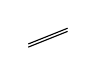
\begin{tikzpicture}\draw (0,0)--(.5,.2);\draw (0,-.04)--(.5,.16);\end{tikzpicture}}}
\noindent 10) \uline{Application 2} Autodualité de
\deleted{$\unsure{H^1}$}
$W_n(K)/F^mW_{\unsure{n}}(\unsure{K})$

\noindent 11) \uline{Application} 3 Cohomologie des V.A.

\noindent 12) L'isom de Lang \deleted{pour \unsure{un corps}}
\inserted{(sur corps $k$ fini)}

\noindent 13) \uline{Application} 4 Dualité de Tate.

\noindent 14) \uline{Compléments en égales caractéristiques}
\inserted{\uline{Théorie de Rosenlicht locale}}
\[
H^i(K,\unsure{\sigma|\gamma}_K)\simeq\operatorname{Ext}^i_{k\text{-gr}}(J_{K/k},\unsure{\sigma|\gamma})
\]
\margin{?}
pour $i>0$, tt $k$-groupe $\unsure{\sigma|\gamma}$, grâce à l'\unsure{isom}
canonique de $J(K)/J(V)'$.

\deleted{\[
\unsure{\mu_p\otimes\mu_p}\\
\unsure{\underline{\operatorname{Hom}}(\mu_p\otimes\mu_p,G_m)}
\unsure{\simeq}\unsure{\operatorname{Hom}(\mu_p,\mathbb Z/p\mathbb Z)}
\]}
\[
\left[\begin{array}{ll}
\uline{\text{Lang}}:&\text{\unsure{géom.} des corps de classes \unsure{prim.} globale par Rosenlicht + Lang}\\
\uline{\text{Serre}}:&\text{\unsure{géométrisation|généralisation} des corps de classes locale}\\
\uline{\text{Tate}}:&\text{Dualité de la cohomologie des V.A. sur un}\\
&\text{corps \unsure{p adique}.}
\end{array}\right.
\]
\mspage{101}

\scanpage{103}
\mspage{102}
\mspage{21.}
\uline{Remark}\quad Since $J(P_k)$ is a finite group(1.5), $J(\xi)$ is of
finite order $q_k$ say. Then (6.2) asserts that $Q_{n,k}$ is S-reducible
if and only if $n\equiv0\bmod q_k$. In particular, values of $n$ for
which $Q_{n,k}$ is S-reducible always exist. Theorem (6.2) includes one
of the main results of [10]. Most of the other results of [10] are
simple consequences of (6.1) (6.2) and the results of \S1--3.

The interest of the spaces $Q_{n,k}$ lies in their relation to the
Stiefel manifolds $O_{n,k}=O_n/O_{n-k}$ as explained in [10]. There is
a commutative diagram of maps
\diagram{\begin{tikzcd}[column sep=small,row sep=small]
Q_{n,k}\arrow[rr,"i"]\arrow[dr,"\rho"']&&O_{n,k}\arrow[dl,"\pi"]\\
&S^{dn-1}&
\end{tikzcd}}
where $i$ is an inclusion induced by the inclusion $Q_n\subset O_n$,
$\pi$ is the fibre map $O_{n,k}\longrightarrow O_{n,1}=S^{dn-1}$ and
$\rho$ is the ``cofibre map'' $Q_{n,k}\longrightarrow Q_{n,1}=S^{dn-1}$.
By determining the connectivity of the pair $(O_{n,k},Q_{n,k})$ James
in (8.2) of [10] proves:

LEMMA (6.3) $Q_{n,k}$ \uline{is reducible if and only if}
$O_{n,k}\longrightarrow S^{\unsure{3n-1|dn-1}}$ \uline{has a cross-section
and, for} $F=R$, $n\geq2k$ \uline{or} $k=1$.

Now $Q_{n,k}$ is r-connected where $r=d(n-k+1)-2$. Hence by (2.6) of [17]
\[
\pi_{dn-1}(Q_{n,k})\longrightarrow\Pi^S_{dn-1}(Q_{n,k})
\qquad\text{(the stable group)}
\]
is an epimorphism for $2r\geq dn-2$ i.e. for
$n\geq2(k-1)+\frac2d$. Now from cohomology considerations $Q_{n,k}$
cannot be reducible unless $n\geq2k$, or $k=1$. Hence we have

LEMMA (6.4) $Q_{n,k}$ \uline{is reducible if and only if it is
S-reducible and} $n\geq2k$ \uline{or} $k=1$.

By (6.2), if $Q_{n,k}$ is S-reducible, $n$ is a multiple of $q_k$
(the order of $J(\xi)$ in $J(P_k)$). The results of [3] or [4] show that
in the complex and quaternionic cases $q_k\geq2k$ for $k>1$. Hence from
(6.2) (6.3) and (6.4) we obtain finally:

THEOREM (6.5) \uline{In the real case suppose} $n\geq2k$. \uline{Then}
$O_{n,k}\longrightarrow S^{dn-1}$ \uline{has a cross-section if and
only if} $n$ \uline{is a multiple of} $q_k$, \uline{where} $q_k$
\uline{in the order of} $J(\xi)$ \uline{in} $J(P_k)$

In one respect this result is weaker than results of [9]. In the real
case we make no assertion for the case $n<2k$ whereas James

\scanpage{104}
\diagram{\begin{tikzcd}k&V\arrow[l]\arrow[r]&K\end{tikzcd}}
\margin{\figure{\begin{tikzpicture}\node[draw,ellipse,rotate=15]{\uuline{parfait} ?};\end{tikzpicture}}}
\diagram{\begin{tikzcd}[column sep=large]
\mathcal K\operatorname{Gr}_K\arrow[d,"T"'] &
\text{complexes finis de \deleted{\unsure{quasi}} $K$-groupes \deleted{\unsure{alg}}}\\
\unsure{K|\mathcal K}\operatorname{QuGr}_k & \text{complexes finis de $k$-quasi-groupes}
\end{tikzcd}}
\margin{\deleted{$\unsure{T^0}$}}
\margin{[Coh de $K$. \uline{ne se calcule pas} galoisiennement]}
\margin{[Coh. de $k$ se calcule galoisiennement, \deleted{\unsure{et}}
ne change pas en remplaçant $k$ par une clôture \unsure{parfaite}]}
\[
T(G)=T^0_{\unsure{a}}e(G)
\]
\[
\Gamma^*_{\unsure{K}}G\simeq\Gamma^0_K e(G)
\simeq\Gamma^0_k T^0e(G)\simeq\Gamma^*_kT(G)
\]
\deleted{\unsure{Question}}\figure{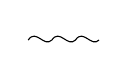
\begin{tikzpicture}\draw(0,0)..controls(.1,.15)and(.2,-.1)..(.3,0)..controls(.4,.15)and(.5,-.1)..(.6,0)..controls(.7,.15)and(.8,-.1)..(.9,0);\end{tikzpicture}}
\noindent (i) $T^0$ transforme injectifs en $\Gamma^0_k$-acycliques ??

\noindent (ii) $T^0$ de dim coh. $\leq2$
[et même $\leq1$ si on \deleted{\unsure{excepte}}\inserted{exclut}
les composantes de type $\mathbb Z$]

\noindent (iii) $T^*$ commute à ``\uline{l'extension du corps résiduel $k$}''.

i.e est ``de nature géométrique'' ;
\diagram{\begin{tikzcd}[column sep=large,row sep=small]
\underline{\underline H}^*(K,G^\bullet) &
H^p(k,\underline{\underline T}^{\unsure{q}}(G^\bullet))\arrow[l,Rightarrow]\\
\underline{\underline H}^*(k,T(G))\arrow[u,equal]&
\end{tikzcd}}
\[
\left[\begin{aligned}
\underline{\underline{\operatorname{Ext}}}^{\unsure{\bullet|*}}_{K\text{-gr}}(F,G)
&\Longleftarrow H^p(k,\underset{\sim}{\underline{\operatorname{Ext}}}^q_{K/k}(F,G))\\
&\Longleftarrow H^p(K,\underset{\sim}{\underline{\operatorname{Ext}}}^q_K(F,G))
\end{aligned}\right.
\]
\mspage{103}

\scanpage{105}
\mspage{104}
\uline{REFERENCES}

\noindent 1. M.F. Atiyah, ``Complex analytic connections in fibre bundles''
Trans. Amer. Math. Soc.

\noindent 2. M.F. Atiyah and F. Hirzebruch, ``Riemann-Roch theorems for
differentiable manifolds'', Bull. Amer. Math. Soc. 65 (1959\unsure{)}
p.276-281.

\noindent 3. M.F. Atiyah and J.A. Todd ``On complex Stiefel manifolds'',
Proc. Camb. Phil. Soc. (1960)

\noindent 4. A. Borel and J-P. Serre. ``Groupes de Lie et puissances
réduites de Steenrod'', American J. of Math. 75 (1953) 409-48.

\noindent 5. S.S. Cairns, ``On the triangulation of regular loci''.
Ann. of Math. 35 (1934) 579-87.

\noindent 6. A. Dold and R. Lashof, ``Principal quasifibrations and fibre
homotopy equivalence of bundles'' Illinois J. of Math. 3 (1959) 285-305.

\noindent 7. F. Hirzebruch, ``A Riemann-Roch theorem for differentiable
manifolds'', Séminaire Bourbaki (1959) No.177.

\noindent 8. I.M. James, ``The intrinsic join'', Proc. London Math. Soc
(3), 8 (1958) 507-35.

\noindent 9. I.M. James, ``Cross-sections of Stiefel manifolds'', ibid
536-47.

\noindent 10. I.M. James, ``Spaces associated with Stiefel manifolds'',
ibid (3) 9 (1959) 115-40.

\noindent 11. J. Milnor and E.H. Spanier (to appear)

\noindent 12. J.P.Serre, ``Homologie singulière des espaces fibrés'',
Ann. of Math.54 (1951) 425-505.

\noindent 13. E.H. Spanier and J.H.C. Whitehead ``Duality in homotopy
theory'' Mathematika, 2 (1955) 56-80.

\noindent 14. N. Steenrod ``The topology of fibre bundles''
(Princeton Univ. Press, 1951).

\noindent 15. R. Thom, ``Espaces fibrés en sphères et carrés de Steenrod'',
Ann. Sco. Ecole Norm. Sup. 69 (1952) 109-182.

\noindent 16. R. Thom, ``Quelques propriétés globales des variétés
differentiables Comment. Math. Helv. 28 (1954) 17-86.

\scanpage{106}
\diagram{\begin{tikzcd}[column sep=huge,row sep=huge]
K^-_{\unsure{fini}}(K)^\circ\arrow[r,"D"]\arrow[d,"T"']
\arrow[dr,phantom,"\substack{\uline{\text{Théorie de}}\\\uline{\text{dualité gén.}}\quad\simeq}"]&
K^+_{\unsure{fini}}(K)\arrow[d,"T(-1)"]\\
K^-(k)'{}^\circ\arrow[r,dash,"\Delta"]\arrow[d,"S"']
\arrow[dr,phantom,"\substack{\uline{\text{Frobenius}}\\\uline{\text{-Lang}}\quad\simeq}"]&
K^+(k)'\arrow[d,"S(-1)"]\\
K^-\deleted{\unsure{\mathcal G}}\mathcal C^\circ\arrow[r,"\Theta"]&K^+\mathcal C
\end{tikzcd}}
\[
\left\{\begin{array}{ll}
D&\text{dualité de Cartier}\\
\Delta&\text{dualité de Serre}\\
\Theta&\text{dualité de \unsure{Pontryagin}}
\end{array}\right.
\]
$\mathcal C$ groupes top. abéliens loc. compacts tt discontinus

(le $'$ indique qu'on n'admet pas de composantes $\mathbb Z$)

$k$ corps \uuline{fini}
\[
\left\{\begin{array}{ll}
T&\text{foncteur Greenberg-\unsure{Néron}-Grothendieck}\\
S&\text{foncteur }\Gamma_k
\end{array}\right.
\]
Comment obtient on le carré du bas ?

\deleted{\unsure{Remarque}}
\diagram{\begin{tikzcd}[column sep=small,row sep=small]
\operatorname{Ext}^i_{k\text{gr}}(G,\mathbb Z/n\mathbb Z)\arrow[r,equal,"\sim"]&
\operatorname{Ext}^{i-1}_{\mathrm{gr.top.}}(SG,\mathbb Z/n\mathbb Z)\arrow[d,equal]\\
&\operatorname{Ext}^i(SG,\mathbb Z/n\mathbb Z(-1))
\end{tikzcd}}
\diagram{\begin{tikzcd}
G\arrow[r,"\text{deg }i"]&\mathbb Z/n\mathbb Z
\end{tikzcd}}
\diagram{\begin{tikzcd}
SG\arrow[r,"\text{deg }i"]&S(\mathbb Z/n\mathbb Z)\arrow[r,"\text{degré }0"]&
\mathbb Z/n\mathbb Z(-1)
\end{tikzcd}}
\[
\begin{aligned}
\underline{\underline{\operatorname{Ext}}}^{0}_{\mathrm{gr.top}}
(\unsure{S(\mathbb Z/n\mathbb Z)|\{\mathbb Z/n\mathbb Z\}}\deleted{(-1)},\mathbb Z/n\mathbb Z(-1))
&=\underline{\underline{\operatorname{Ext}}}^{-1}_{k\mathrm{gr}}
(S(\mathbb Z/n\mathbb Z),\mathbb Z/n\mathbb Z)\\
&=\operatorname{Hom}(H^{\unsure{1}}S(\mathbb Z/n\mathbb Z),\mathbb Z/n\mathbb Z)
\simeq\mathbb Z/n\mathbb Z\quad !
\end{aligned}
\]
\margin{\figure{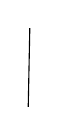
\begin{tikzpicture}\draw (0,0)--(.02,1);\end{tikzpicture}}}
\deleted{$\unsure{\mathbb Z}$}
\mspage{105}

\scanpage{107}
\[
\boxed{H^i(A)\times H^{2-i}(B)\mathrel{-}H^2(K,G_m)}
\]
\[
H^{\unsure{1}}({}_nA)\longrightarrow
\]
\[
\underline{\varinjlim}
\]
\[
H^{\unsure{1}}(K,A)
\]
\[
\operatorname{Ext}^i_{k\mathrm{gr}}(G,H)\simeq
\operatorname{Ext}^{i-2}(R\Gamma G,H)=\operatorname{Hom}(H^{2-i}(\unsure{1}
\]
\[
H^i(
\]
\deleted{$\unsure{H^i(}$}
\[
\operatorname{Ext}^i_{k\mathrm{gr}}(G,\mathbb Z/n\mathbb Z)\simeq
\operatorname{Hom}(H^{1-i}(K,G),\mathbb Z/n\mathbb Z)
\]
\[
\operatorname{Ext}^i_{k\mathrm{gr}}(G,\mathbb Q/\mathbb Z)\simeq
\operatorname{Hom}(H^{1-i}(K,G),\unsure{\mathbb Q/\mathbb Z})
\]
\deleted{1) $G$ \unsure{grp} fini}

\uline{$1^\circ$}) $G$ \uline{\unsure{grp} fini ordinaire} $\mathbb Z/n\mathbb Z$
\[
\deleted{\unsure{H^{1-i}}(\quad H^i(K,G)\times H^{\unsure{1-i}}(K,\widehat G}
\]
\[
H^i(K,\mathbb Z/n\mathbb Z)\times H^{1-i}(K,\mathbb Z/n\mathbb Z)
\unsure{\mathrel{-}|\longrightarrow}\mathbb Q/\mathbb Z
\]
\[
\mathbb Z/n\mathbb Z\qquad\mathbb Z/n\mathbb Z
\]
\mspage{106}

\scanpage{108}
\mspage{107}\margin{\figure{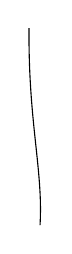
\begin{tikzpicture}\draw(0,0)..controls(.04,.7)and(-.15,1.3)..(-.14,2.5);\end{tikzpicture}}}
\deleted{
\uline{Corollaire} \unsure{4|2}.9.10. Soit $f:X\longrightarrow Y$ un morphisme \deleted{de}
\inserted{de type fini,} \deleted{\unsure{propre}} où $Y$ loc. noeth., $y\in Y$, on suppose
$f$ \unsure{univ.} ouvert en les \unsure{pts} de $X_y$, et $X_y$ séparable.
\deleted{Alors, la fonction $\unsure{y}\mapsto\unsure{\pi_0(y)}$}
\inserted{Pour tt $z\in\unsure{Z|Y}$, soit $\pi(z)=\unsure{\mathrm{nb}^{\mathrm{re}}}$ de}
\unsure{composantes} connexes \unsure{géom} de $X_z$. Alors la fonction
$z\mapsto\unsure{\pi(z)}$ est
\deleted{\unsure{continue} \unsure{en} \unsure{y}}
\inserted{\unsure{$\frac12$} \unsure{continue}}
\unsure{en} \deleted{\unsure{un} \unsure{voisinage}} de $y$.
[elle est continue en $y$].

\deleted{La \deleted{\unsure{fonction}} \unsure{définie} \unsure{ci-dessus} est ``$\frac12$ continue
\unsure{semi-inférieurement}'', par la ``\unsure{th.} de connexité''.}

\deleted{\unsure{Il reste} \illegible{4} \unsure{qu'elles sont}
\unsure{les composantes} \unsure{supérieures} \unsure{à} \unsure{ceux}
\unsure{connexes} (\unsure{comme} elles sont \unsure{constr.}).}

Pour \unsure{tout} \unsure{pt} géom $y'$ de $y$,
on a $\pi(y)\geq\pi(y')$. La \unsure{propriété}
\unsure{précitée} nous ramène alors
au cas où $Y$ est le spectre d'un
anneau de valuation discrète, et où
les \unsure{composantes} connexes de $\unsure{X_0},\unsure{X_1|X_\eta}$
\unsure{sont} géométriques. On peut \unsure{ainsi}
\unsure{supposer} $X$ connexe, \unsure{alors}
$\unsure{X_1|X_\eta}$ est connexe,
\deleted{$\unsure{X_0}$ \unsure{a} \unsure{fini}}
donc \deleted{$\pi(\unsure{X_0})$} $\pi(X_1)=1$,
\deleted{\unsure{donc}} \uline{et}
\uline{comme} $X_0\neq\varnothing$, on a fini.
}
\margin{\figure{\begin{tikzpicture}
\draw (0,0)--(0,1.5);\fill (0,0) circle (.04);
\end{tikzpicture}}}
\margin{\figure{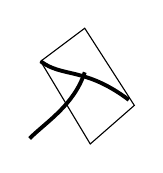
\begin{tikzpicture}[scale=.7]
\draw (0,1.5)--(.8,2.1)--(1.7,.7)--(.9,0)--cycle;
\draw[line width=1.4pt] (0,1.5)..controls(.4,1.2)and(.8,1.4)..(1.6,.8);
\draw[line width=1.4pt] (.8,1.3)..controls(.6,.7)and(.1,.4)..(-.2,.1);
\end{tikzpicture}}}
\margin{\figure{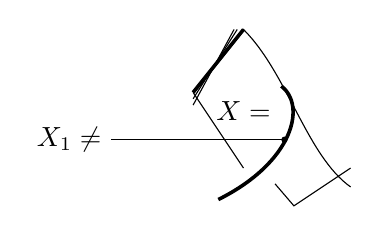
\begin{tikzpicture}[scale=.8]
\draw (0,1.7)--(.8,2.7)..controls(1.5,2)and(1.8,.7)..(2.5,.2);
\draw (0,1.7)--(.8,.5);\draw (1.3,.25)--(1.6,-.1)--(2.5,.5);
\draw[line width=1.3pt] (0,1.7)--(.8,2.7);
\draw (0,1.6)--(.7,2.7);\draw (0,1.5)--(.65,2.7);
\draw[line width=1.3pt] (.4,0)..controls(1.6,.6)and(1.8,1.5)..(1.4,1.8);
\draw (-1.3,.95)--(1.45,.95);\fill (1.45,.95) circle (.05);
\node[left] at(-1.3,.95){$X_1\neq\varnothing$};
\node at(.8,1.4){$\unsure{X=\varnothing}$};
\end{tikzpicture}}}
\margin{\figure{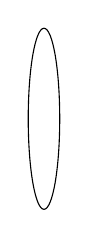
\begin{tikzpicture}\draw (0,0) ellipse (.2 and 1.15);\end{tikzpicture}}}
\deleted{\diagram{\begin{tikzcd}[column sep=small,row sep=large]
0\arrow[r]\arrow[dr,dash,bend right=30]&
N\arrow[r]\arrow[d,dash,bend right=20]&
M\arrow[r,dash]\arrow[d,dash,bend right=15]&
M/N\arrow[r,dash]\arrow[d,dash,bend left=25]&0\arrow[dl,dash,bend left=35]\\
0\arrow[r,dash]&N'+N\arrow[r,dash]&M'+M\arrow[r]&P'+P\arrow[r,dash]&0
\end{tikzcd}}}
\margin{\unsure{Lem} \unsure{d'homologie}}
\margin{\figure{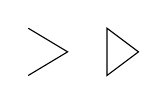
\begin{tikzpicture}\draw (0,0)--(.5,.3)--(0,.6);\draw (1,0)--(1.4,.3)--(1,.6)--cycle;\end{tikzpicture}}}

\scanpage{109}
\uline{$2^\circ$}) $G=\mu_p$
\[
\underline{\operatorname{Ext}}^i_{k\mathrm{gr}}(G,\unsure{\mathbb Q/\mathbb Z})=
\left\{\begin{array}{l}0\\0\\0\\0\end{array}\right.
\]
\deleted{$H^0(k,\mu)$}\qquad $\mathbb Z/n\mathbb Z\quad\mu_p$
\[
\deleted{H^i}\qquad K^*/\unsure{k^{*p}|K^{*p}}
\]
\[
H^1(k,\mu_p)\qquad k^*/k^{*p}
\]
\[
H^i(k,G_m)=
\]
\diagram{\begin{tikzcd}k^*\arrow[r,"p"]&k^*\end{tikzcd}}
\figure{\begin{tikzpicture}[scale=.6]
\draw (0,2.5)..controls(-.2,.7)and(0,0)..(1,0)--(2.8,0)
..controls(4,0)and(4,1)..(4,1.8)..controls(4,2.2)and(7.5,2.1)..(8.5,2.5);
\end{tikzpicture}}
$3^\circ)$ $G=\alpha_p$
\[
x^p
\]
$3^\circ)$ $G=G_m$
\[
\underline{\operatorname{Ext}}^i(G_m,\mathbb Q/\mathbb Z)=
\left\{\begin{array}{l}0\\(\text{racines de l'unité})^\vee\\0\\0\end{array}\right.
\]
\[
1
\]
\[
\underline{\underline{\operatorname{Ext}}}^i_{k\mathrm{gr}}(G_m,\mathbb Q/\mathbb Z)=
H^{i-1}(k,\text{racines de }\unsure{1})^{\unsure{\vee|'}}
\longrightarrow\left\{\begin{array}{l}0\\\unsure{\text{racines de l'unité}}\\0\\0\end{array}\right.
\]
\margin{$1$}
\deleted{$k^*$}
\[
H^i(k,G_m)=\left\{\begin{array}{l}k^*\\0\\0\\\unsure{0}\\\unsure{0}\end{array}\right.
\]
\[
\operatorname{Ext}(G_m,\deleted{\mathbb Z/n\mathbb Z}{}_n\mu)=\mathbb Z/n\mathbb Z
\]
\[
\operatorname{Ext}(G_m,\mathbb Z/n\mathbb Z)\simeq{}_n\mu^\vee
\]
\[
\operatorname{Ext}(G_m,\unsure{\mathbb Z_{(\to)1}|\mathbb Z_{(\infty)1}})
\simeq\underset{n}{\underline{\lim}}\,{}_n\mu^\vee
\]
\[
\operatorname{Hom}(\Pi_\bullet(G_m),\mathbb Q/\mathbb Z)
\]
\margin{$\boxed{\begin{array}{c}
\operatorname{Ext}_{k\mathrm{gr}}(G_m,\mathbb Q/\mathbb Z)\\[1em]
\uline{\unsure{est de}}\quad k^*
\end{array}}$}
\margin{$\Vert\quad\operatorname{Hom}(G_m(k),\mathbb Q/\mathbb Z)$}
\mspage{108}

\scanpage{110}
IV 7 Oubli au n\textsuperscript{o} 7.6.

\uline{Proposition} 6.7. Soient $f:X\longrightarrow Y$ un morphisme
\deleted{de présentation finie} \deleted{et} propre,
\inserted{avec $Y$ loc. noeth.,}
$F$ un Module \deleted{de présentation finie} \inserted{cohérent}
sur $X$. \inserted{de support $X$,} Pour tout $y\quad Y$,
Soit $\ell(y)$ la somme des \deleted{long} multiplicités \deleted{tota}
géométriques totales \inserted{sur $k(y)$} de
$F_y$ en les points maximaux de $\operatorname{supp}F_y$.
\inserted{On suppose $f$ univ. ouvert en les pts maximaux de $X_{y_0}$,
et $F_{y_0}$ sans \unsure{idéaux} premiers ass. immergés}
Alors la fonction $\unsure{z|y}\mapsto\ell(\unsure{z|y})$ sur
$Y$ est semi-continue supérieurement\inserted{en $y_0$}.
\margin{?}

Le procédé breveté nous ramène au cas où $Y$ est noethérien. On sait
(réf) que la fonction $\ell$ est constructible, il reste donc (réf) à prouver
que $y\in\overline{y'}$ implique $\ell(y)\geq\ell(y')$. Le procédé habituel nous permet
alors de nous ramener au cas où $Y$ est le spectre d'un anneau de valuation
discrète, dont $y$ ($y'$) est le point fermé (générique), et \deleted{\unsure{à prouver}}
à prouver dans ce cas l'inégalité correspondante sur les longueurs:

\uline{Lemme} 6.8. Soit $f:X\quad Y$ un morphisme propre, avec $Y$ spectre d'un anneau
de valuation discrète, $F$ un Module cohérent sur $X$, \inserted{de support $X$,}
$F_0$ et $F_1$ les \deleted{fibr}
Modules induits sur la fibre spéciale resp. la fibre générique, $x_i$
($x'_j$) les points maximaux de $\operatorname{supp}F_0$ ($\operatorname{supp}F_1$).
\inserted{(Supposons que tt comp. de $X$ domine $Y$ et $F_0$ soit $(S_1)$.)}
Alors on a
\[
\operatorname{long} F_{0\,x_i}\unsure{\geq|>}\sum_i\operatorname{long}F_{1\,x'_j}
\]
Si l'inégalité est vérifiée, alors $F$ est plat sur $Y$ aux points \deleted{\unsure{génériques}} \deleted{\unsure{que}}
maximaux de $\operatorname{supp}F_0$, \deleted{donc toute composante de $\operatorname{supp}F$ domine $Y$,}

Soit $t$ une uniformisante pour $V=\underline O_{Y,y}$, soit $N$ le sous-Module
de $F$ réunion des annulateurs des $t^n$, donc on a une suite exacte
\[
0\mathrel{-}N\mathrel{-}F\mathrel{-}G\mathrel{-}0
\]
d'où une suite exacte (grâce au fait que $t$ est $G$-régulier):
\[
0\mathrel{-}N/tN\mathrel{-}F/tF\mathrel{-}G/tG\mathrel{-}0
\]
\unsure{Qela|Cela} montre que les deux sommes \deleted{pour} relatives à $F$ qu'il s'agit de
comparer, s'obtiennent en ajoutant les sommes analogues pour $N,G$.
Comme $N_1=0$, pour prouver notre inégalité, il suffit donc de
prouver l'inégalité analggue pour $G$; et on ne peut avoir égalité
que si $N/tN$ \deleted{est} $=N_0$ est nul aux points maximaux de $\operatorname{supp}$
\unsure{$\cdots$}

\margin{\figure{\begin{tikzpicture}[x=.5cm,y=.5cm]
\draw (0,0)..controls(-.1,2)and(.3,9)..(.9,11);
\draw (4,-1)..controls(4.7,1)and(3.5,8)..(6,15);
\draw (8,0)..controls(8.5,3)and(6.8,7)..(7.5,12);
\end{tikzpicture}}}

\margin{N.B. J'ignore si les assertions sont vraies si on ne
suppose pas déjà $F$ plat$/Y$ aux pts maximaux
de $X_y$. Question liée: $A$ anneau local noeth., $M$ module de
type fini sur $A$, $t\in A$, $\unsure{t\notin\mathfrak p}$\deleted{\unsure{minimal}} pour tt $\mathfrak p$ associé,
on suppose $\operatorname{supp}M=\operatorname{Spec}A$, $\dim\unsure{A/\mathfrak p_0}=1$,
prouver $\mathfrak m\in\operatorname{Ass}M/tM$ !}
\mspage{109}

\scanpage{112}
\diagram{$\begin{array}{c|c}
\begin{gathered}
\mu_n\qquad\deleted{\unsure{(n,p)\neq1}}\ (n,p)=1\\
\begin{tikzcd}[row sep=small]\phantom{\mu_n}\arrow[d,squiggly]\\
\left[\operatorname{Grbg}(G_m)\xrightarrow{n}\operatorname{Grbg}(G_m)\right]\end{tikzcd}\\
[\,0\qquad1\,]\\
\figure{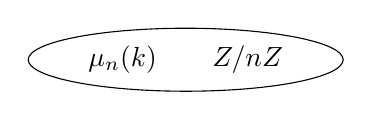
\begin{tikzpicture}\draw (0,0) ellipse (2 and .4);\node at(0,0){$\mu_n(k)\qquad\mathbb Z/n\mathbb Z$};\end{tikzpicture}}
\end{gathered}
&\begin{gathered}
\mathbb Z/n\mathbb Z\qquad(n,p)=1\\
\begin{tikzcd}[row sep=small]\phantom{\mathbb Z/n\mathbb Z}\arrow[d,squiggly]\\
\deleted{\mathbb Q/\mathbb Z\xrightarrow{n}\mathbb Q/\mathbb Z}\end{tikzcd}\\
0\qquad1\\
\figure{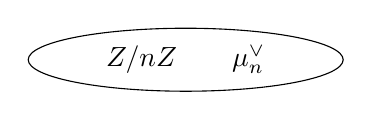
\begin{tikzpicture}\draw (0,0) ellipse (2 and .4);\node at(0,0){$\mathbb Z/n\mathbb Z\qquad\mu_n^\vee$};\end{tikzpicture}}
\end{gathered}\\\hline
\begin{gathered}
\begin{tikzcd}[row sep=small]\mu_p\arrow[d,squiggly]\\
\operatorname{Grbg}(G_m)\arrow[r,"p"]&\operatorname{Grbg}(G_m)\end{tikzcd}\\
[\,0\qquad1\,]\\
\figure{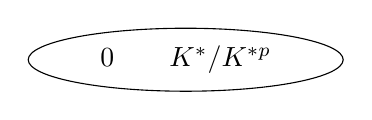
\begin{tikzpicture}\draw (0,0) ellipse (2 and .4);\node at(0,0){$0\qquad K^*/K^{*p}$};\end{tikzpicture}}
\end{gathered}
&\begin{gathered}
\begin{tikzcd}[row sep=small]\mathbb Z/p\mathbb Z\arrow[d,squiggly]\\
\operatorname{Grbg}(G_a)\arrow[r,"\wp"]&\operatorname{Grbg}(G_a)\end{tikzcd}\\
\figure{\begin{tikzpicture}\draw (0,0) ellipse (3.4 and .55);\node at(0,0){$\mathbb Z/p\mathbb Z\quad\underbrace{H^1(K,\mathbb Z/p\mathbb Z)}_{\substack{\text{cf corps de}\\\text{classe local}}}=\unsure{K^+/\wp K^+}$};\end{tikzpicture}}\\
\operatorname{Ext}^{0}(\unsure{K^*/K^{*p}},\mathbb Q/\mathbb Z)\qquad
\operatorname{Ext}_{\unsure{i}}(\unsure{K^*/K^{*p}},\mathbb Q/\mathbb Z)
\end{gathered}\\\hline
\begin{gathered}
\begin{tikzcd}[row sep=small]\alpha_p\arrow[d,squiggly]\\
\operatorname{Grbg}(G_a)\arrow[r,"\text{Frob}"]&\operatorname{Grbg}(G_a)\end{tikzcd}\\
\figure{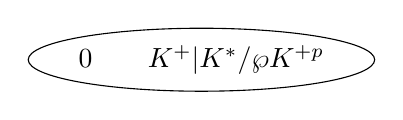
\begin{tikzpicture}\draw (0,0) ellipse (2.2 and .4);\node at(0,0){$0\qquad\unsure{K^+|K^*}/\deleted{\unsure{\wp}}K^{+p}$};\end{tikzpicture}}
\end{gathered}
&\begin{gathered}
\begin{tikzcd}[row sep=small]\alpha_p\arrow[d,squiggly]\\\unsure{\varsigma}\end{tikzcd}\\
\figure{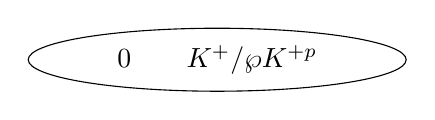
\begin{tikzpicture}\draw (0,0) ellipse (2.4 and .4);\node at(0,0){$0\qquad K^+/\deleted{\unsure{\wp}}K^{+p}$};\end{tikzpicture}}\qquad-
\end{gathered}\\\hline
\begin{gathered}
G_m\\
??\quad\figure{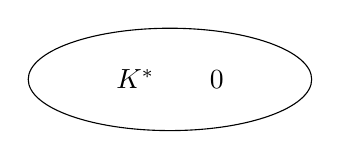
\begin{tikzpicture}\draw (0,0) ellipse (1.8 and .65);\node at(0,0){$K^*\qquad0$};\end{tikzpicture}}\\
\mathbb Z
\end{gathered}
&\begin{gathered}
\mathbb Z\qquad??\\
\figure{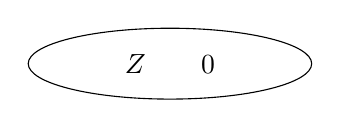
\begin{tikzpicture}\draw (0,0) ellipse (1.8 and .45);\node at(0,0){$\mathbb Z\qquad0$};\end{tikzpicture}}
\quad+H^1(K,\mathbb Q/\mathbb Z)
\end{gathered}
\end{array}$}
\figure{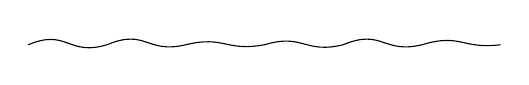
\begin{tikzpicture}[x=.5cm,y=.3cm]
\draw (0,0)..controls(1,.7)and(1,-.5)..(2,0)..controls(3,.7)and(3,-.4)..(4,0)
..controls(5,.4)and(5,-.3)..(6,0)..controls(7,.5)and(7,-.4)..(8,0)
..controls(9,.7)and(9,-.4)..(10,0)..controls(11,.5)and(11,-.2)..(12,0);
\end{tikzpicture}}
\mspage{111}

\scanpage{113}
\deleted{
\unsure{ou}, \inserted{pour tt $x\in X$,} \deleted{\unsure{des}}\inserted{un}
\unsure{élément} \deleted{\unsure{de $\mathcal G_x$}}
$\lambda_x\in\gamma(\deleted{\unsure{\xi}}\xi_x,\xi)
=\operatorname{Is}_K(K(\unsure{O_\xi}),K(\unsure{O_x}))
=\operatorname{Is}_K(K',K(\unsure{O_x}))$,
i.e. donnons nous un \unsure{point-g.} \unsure{certifié}
\deleted{\unsure{de}} de $K'$ au dessus de $x$.

On a une famille d'homomorphismes
\diagram{\begin{tikzcd}[column sep=large]
\varphi_x:\operatorname{Gal}(\overline K_x/K_x)\arrow[r,"\text{épim.}"]&
\operatorname{Gal}(K'/K_x^{\unsure{\mathrm{dec}}})\subset\operatorname{Gal}(K'/K)
\end{tikzcd}}
(homomorphismes de réciprocité).
\margin{application de réciprocité i.e. \unsure{logarithme} local}
\deleted{\unsure{Le groupe}} \deleted{\unsure{Donne}}
\uline{Le groupe \inserted{\uuline{invariant} dans $\operatorname{Gal}(K'/K)$}
engendré par les} $\operatorname{Im}\varphi_x$
\uline{est le} \deleted{\uline{plus gr.}\ \unsure{sous-gr.}}
\inserted{groupe de \unsure{galois|Galois}}
$\operatorname{Gal}(K'\deleted{\unsure{{}_x^{\mathrm{dec}}}}/K_X^{\unsure{\mathrm{D\acute ec}}})$,
\uline{où} $K_X^{\unsure{\mathrm{D\acute ec}}}$ \uline{est la plus grande sous-extension}
\inserted{galoisienne} \uline{de} $K'$, \uline{de} $K$, \uline{qui est complètement}
\deleted{\unsure{en}} \uline{décomposée sur chaque} \deleted{$x\in X$} $x\in X$.

\unsure{De même}, quand on prend les hom. induits par les $\varphi_x$
\diagram{\begin{tikzcd}[column sep=large]
\operatorname{Gal}(\overline K_x/\overline K_x^{i})\arrow[r,"\text{épim}"]&
\operatorname{Gal}(K'/K_x^i)\subset\operatorname{Gal}(K'/K)
\end{tikzcd}}
\uline{on trouve comme groupe \inserted{\uuline{invariant} \unsure{par}} fermé engendré
par les} $\varphi_x(\operatorname{Gal}(\overline K_x/\overline K_x^I))$ \uline{le groupe
de Galois} $\operatorname{Gal}(K'\deleted{\unsure{{}_x}}/K_X^{\unsure{\mathrm{Iner}}})$,
\uline{où} $K_X^{\unsure{\mathrm{Iner}}}$ \uline{est la}
\deleted{\unsure{plus}}
\uline{plus grande sous-extension de} $K'$ \uline{non ramifiée
sur $X$}.
}
\mspage{112}

\scanpage{114}
\[
\mu_n^\vee\qquad\mathbb Z/p\mathbb Z\qquad1
\]
\[
\operatorname{Ext}
\]
\[
\boxed{H^i(K,D(\unsure{\widehat G|G}))\simeq
\operatorname{Ext}^{1-i}(f_*G,\mathbb Q/\mathbb Z)}
\]
\[
A(k)
\]
\[
\underset{\sim}{\operatorname{Ext}}^i(
\]
\[
\operatorname{Ext}^0(A(k),\mathbb Q/\mathbb Z))^{1-i}
\]
\[
\boxed{f_*D(G)\simeq(Tf_*G)\unsure{(-1)|(1)}}
\]
\[
=\operatorname{Ext}^{\unsure{i}}(A,\mathbb Q/\mathbb Z)(k)^{1-i}
\]
\[
H^i(K,D(G))\simeq\operatorname{Ext}^i(f_*G,\mathbb Q/\mathbb Z)
\]
\[
\operatorname{Ext}^{\unsure{1+d-i|1+0-i}}(A,\mathbb Q/\mathbb Z)^{\unsure{1+d-i|1+0-i}}
\]
\figure{\begin{tikzpicture}\draw (0,1.5)..controls(.5,2)and(.2,.7)..(.8,0);\end{tikzpicture}}
\[
\boxed{H^i((T\unsure{f_*}G)(-1))=H^{\unsure{i-1}}(T\unsure{f_*}G)
=\underline{\underline{\operatorname{Ext}}}^{\unsure{i-1}}(f_*G,\mathbb Q/\mathbb Z)}
\]
\margin{\figure{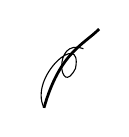
\begin{tikzpicture}\draw[line width=1pt] (0,0)..controls(.2,.7)and(.5,.8)..(.7,1);\draw (0,0)..controls(-.2,.4)and(.5,1)..(.4,.5)..controls(.2,.1)and(.1,.9)..(.5,.75);\end{tikzpicture}}}
\[
\boxed{H^i(K,D(G))\deleted{\unsure{f_*G}}
\overset{\uline{\unsure{1}}}{\overset{\sim}{\longrightarrow}}
\underline{\underline{\operatorname{Ext}}}^{\unsure{i-1}}(f_*G,\mathbb Q/\mathbb Z)}
\]
\[
\operatorname{Ext}^{i-1}(M(-1),\mathbb Q/\mathbb Z)
=\operatorname{Ext}^{\unsure{i}}(M,\mathbb Q/\mathbb Z)(1)^{i-1}
\]
\margin{$\operatorname{Ext}^{i-1}(H_{\deleted{\unsure{\mathrm{coh}}}}^{1-i}(f_*G))$}
\margin{$=\operatorname{Ext}^{\unsure{i}}(\unsure{\gamma}$}
\[
\boxed{H^{\unsure{i+1|p+q}}(K,DG)\Longleftarrow
\operatorname{Ext}^{p}(H^{-q}(K,G),\mathbb Q/\mathbb Z)}
\]
\[
0\longrightarrow\operatorname{Ext}^{1}_{k\mathrm{gr}}(H^{1-i}(K,G),\mathbb Q/\mathbb Z)
\longrightarrow H^{i-1}(K,DG)\longrightarrow
\operatorname{Hom}_{k.\mathrm{gr}}(H^{-i}(K,G),\mathbb Q/\mathbb Z)
\]
\mspage{113}

\scanpage{115}
\mspage{114}
\mspage{III-49}
me de dévissage (II,1,5,cor. du th.3), on est ramené à prouver que
lorsque $X$ est irréductible, il existe \uuline{un} $\underline O_X$-Module cohérent de support
$X$ appartenant à \uuline{$K'$}: en effet, si ce point est établi, on
pourra l'appliquer à toute partie fermée irréductible $Y$ de $X$, car
si $\underline G$ est un $\underline O_Y$-Module cohérent et $j$ l'injection canonique $Y\to X$, on
a $R^q(f\circ j)_*(\underline G)=R^qf_*(j_*(\underline G))$ (G,II,4.9.1), et le corollaire du lemme
de dévissage s'applique.

En vertu du lemme de Chow (II,5,2,cor.1 du th.1), il existe un
préschéma irréductible $X'$ et un morphisme \inserted{\uline{projectif}} surjectif \inserted{\uline{et}} birationnel $g:$
$X'\to X$ tels que $f\circ g:X'\to Y$ soit \uline{projectif}. Comme $X$ est noethérien
\deleted{\unsure{et $g$ fermé}, on en déduit (II,4,6,th.3 (ii)) que $g$ est aussi un morphisme projectif; comme $X$ est noethérien},
$X'$ est isomorphe à un
préschéma $\operatorname{Proj}(\underline S)$, où $\underline S$ est une $\underline O_X$-Algèbre \deleted{\unsure{$g$}} quasi-cohérente
graduée à degrés positifs, engendrée par $\underline S_1$, où $\underline S_1$ est un $\underline O_X$-Module
cohérent (II,4,6,prop.21 (ii)). Le th.1 du \S\ 2,n\textsuperscript{o}2 est applicable
à $g:X'\to X$, et il existe donc un entier $n>0$ tel que \deleted{$\unsure{R^qg_*}$}
$\underline F=g_*(\underline O_{X'}(n))$ soit cohérent et $R^qg_*(\underline O_{X'}(n))=0$ pour tout $q>0$; en outre,
comme $g$ est birationnel, le support de $\underline F$ contient un ouvert
partout dense de $X$, et comme ce support est fermé\inserted{(FAG,I,2,12,prop.1)}, il est identique
à $X$. D'autre part, comme $f\circ g$ est projectif et $Y$ noethérien,
le \uline{même raisonnement} (II,4,6,prop.21 (ii) et \S\ 2,n\textsuperscript{o}2,th.1) montre
que les $R^p(f\circ g)_*(\underline O_{X'}(n))$ sont cohérents. Cela étant, \deleted{$\unsure{R^pf_*}$}
$R^*(f\circ g)_*(\underline O_{X'}(n))$ est l'aboutissement d'une suite spectrale dont le
terme $E_2$ est donné par $E_2^{pq}=R^pf_*(R^qg_*(\underline O_{X'}(n)))$ (suite spectrale de
Leray; \S\ 0,n\textsuperscript{o}\quad). D'après ce qui précède, on a $E_2^{pq}=0$ pour $q>0$;
on sait alors que \deleted{\unsure{le}} $E_2^{p0}=R^pf_*(\underline F)$ est isomorphe à $R^p(f\circ g)_*(\underline O_{X'}(n))$
(G,I,4.4.1), ce qui achève la démonstration.
\margin{\figure{\begin{tikzpicture}\draw (0,0)--(.15,.15);\draw (.08,.1)--(.22,-.04);\end{tikzpicture}}}

\uline{Corollaire 1 .- Soit} $Y$ \uline{un préschéma localement noethérien. Pour tout}
\uline{morphisme propre} $f:X\to Y$ \deleted{\unsure{noethérien}}, \uline{l'image directe par $f$ de}

\scanpage{116}
\[
H^*(\Delta^2T(A))\Longleftarrow(H^p\Delta^2)(H^q(K,A))
\]
\[
E_2^{pq}=\deleted{\unsure{H^p(\Delta^2H^qA)}}
\left\{\begin{array}{l}0\text{ si }q\neq0,\ p\unsure{\neq|=}q\\\phantom{0}\end{array}\right.
\]
\figure{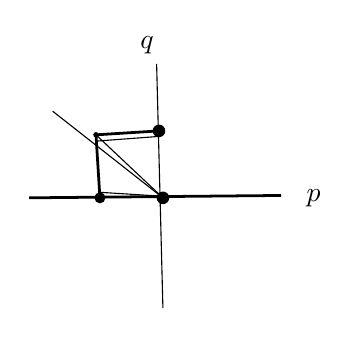
\begin{tikzpicture}
\draw[line width=1pt] (-1.7,0)--(1.5,.03);\node[right] at(1.7,0){$p$};
\draw (0,-1.4)--(-.08,1.7);\node[above] at(-.2,1.7){$q$};
\draw[line width=1pt] (-.8,0)--(-.85,.8)--(-.05,.85);
\draw (-1.4,1.1)--(0,0);\draw (-.85,.8)--(0,0);
\draw (-.85,.72)--(-.05,.78);\draw (-.8,.07)--(0,.02);
\fill (-.8,0) circle (.07);\fill(0,0) circle(.08);\fill(-.05,.85) circle(.08);\fill(-.85,.8) circle(.035);
\end{tikzpicture}}
\[
\left\{\begin{array}{l}
(H^{-1}\Delta^2)(H^0(K,A))\subset\pi_1(A)\\[1em]
(H^0\Delta^2)(H^0(K,A))\\[1em]
(H^0\Delta^2)(H^1(k,A))=H^1(K,A)
\end{array}\right.
\]
\margin{\uline{compact}}
\margin{\deleted{\unsure{qui est}}\inserted{\figure{\begin{tikzpicture}\node[draw,ellipse]{\uline{est le \unsure{plus gr}}};\end{tikzpicture}}}
\uline{\unsure{complété}} de \uline{fini}}

$\Delta T(\mathcal P_\bullet)$ et $T(\mathcal P'_\bullet)$ \uuline{sont $=\unsure{\Delta|0}$.}
\[
\boxed{\underline{\underline{\operatorname{Ext}}}^{0}(\unsure{\mathcal P},\mathbb Q/\mathbb Z)=0}
\]
\[
\operatorname{Ext}(H
\]
\diagram{\begin{tikzcd}
T(\mathcal P')&\Delta T(\mathcal P_\bullet)\arrow[l,Leftarrow]
\end{tikzcd}}
\margin{\figure{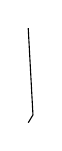
\begin{tikzpicture}\draw (0,1.2)--(.06,.1)--(0,0);\end{tikzpicture}}}

\deleted{\uline{Remarque} 2.7. J'ignore si les conditions
d'équidimensionnalité de 1.1. ii) sont
essentielles; de $=$ dans 2.6.

\uline{Prop.} 2.8. Continuité des Cohen-Macaulay.}
\mspage{115}

\scanpage{117}
\[
A'_0=\mathcal A'\qquad\pi_0(A)\text{ et }\pi_0(B)\text{ duaux}
\]
\[
\boxed{\begin{array}{l}
(3)\quad\left\{\begin{aligned}
H^1(K,A)&\simeq\underline{\operatorname{Ext}}_{k\mathrm{gr}}(\mathcal B,\mathbb Q/\mathbb Z)
\simeq\underline{\operatorname{Ext}}^1_{k\mathrm{gr}}(\mathcal B'{}^0,\mathbb Q/\mathbb Z)
\times\underline{\operatorname{Ext}}_{k\mathrm{gr}}(V,\mathbb Q/\mathbb Z)\\
H^1(K,B)&\simeq\underline{\operatorname{Ext}}_{k\mathrm{gr}}(\mathcal A,\mathbb Q/\mathbb Z)
\simeq\underline{\operatorname{Ext}}^1_{k\mathrm{gr}}(\mathcal A'{}^0,\mathbb Q/\mathbb Z)
\times\underline{\operatorname{Ext}}_{k\mathrm{gr}}(U,\mathbb Q/\mathbb Z)
\end{aligned}\right.\\[1em]
(2)\quad\pi_0(A)\text{ et }\pi_0(B)\text{ duaux (à valeurs dans }\mathbb Q/\mathbb Z)\\[1em]
(1)\quad0\longrightarrow\pi_1(A'_0)\longrightarrow
\end{array}}
\]
\margin{\deleted{\unsure{Vue d'ensemble}}}
\figure{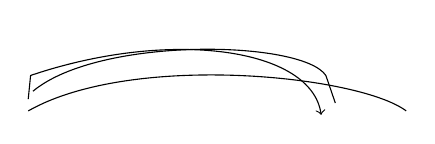
\begin{tikzpicture}[x=.6cm,y=.5cm]
\draw[->] (0,0)--(.05,.6)..controls(3,1.8)and(6,1.3)..(6.2,-.4);
\draw (.1,.2)..controls(1.5,1.6)and(5.8,1.5)..(6.3,.6)--(6.5,-.1);
\draw (0,-.3)..controls(2.2,1.2)and(7,.6)..(8,-.3);
\end{tikzpicture}}
\figure{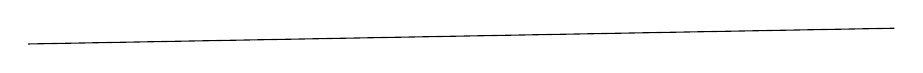
\begin{tikzpicture}\draw (0,0)--(11,.2);\end{tikzpicture}}
\diagram{\begin{tikzcd}
0\arrow[r]&U\arrow[r]\arrow[d,phantom,"\text{unip. connexe}"]&
\mathcal A\arrow[r,dash]&\mathcal A'\arrow[r,dash]\arrow[d,phantom,"\text{sans unip. connexe}"]&0\\
&\phantom{U}&&\phantom{A'}&
\end{tikzcd}}
\[
\mu(A)=2\underbrace{\alpha(A^0)}_{\substack{\text{\unsure{composante}}\\\deleted{\text{multiplicative}}\\\text{abélienne}}}
+\underbrace{\mu(A^0)}_{\substack{\text{comp.}\\\text{multiplicative}}}
\]
\diagram{\begin{tikzcd}[column sep=small]
0\arrow[r,dash]&\operatorname{Ext}^1(\mathcal A'{}^0,\mathbb Q/\mathbb Z)\arrow[r]
\arrow[d,phantom,"(\mathbb Q/\mathbb Z)^{\unsure{\mu(A)}}"]&
\operatorname{Ext}^1(\mathcal A,\mathbb Q/\mathbb Z)\arrow[r]\arrow[d,equal]&
\underline{\operatorname{Ext}}(U,\mathbb Q/\mathbb Z)\arrow[r]
\arrow[d,phantom,"\substack{\text{groupe \unsure{proalgébrique}}\\\text{\unsure{unip.} connexe}}"]&0\\
&\phantom{X}&H^1(K,B)&\phantom{X}&
\end{tikzcd}}
\mspage{116}

\scanpage{118}
\deleted{
1. \inserted{Morphismes plats \unsure{etc.}} Changement de base, \deleted{platitude}

2. $\underset{\longleftarrow}{\operatorname{Lim}}$ de préschémas, propriétés constructibles

3. \unsure{(?)} Morphismes réguliers etc. Application à l'algèbre locale.

Pourrait passer au Chap 0 ?

4. Morphismes plats de présentation finie: \unsure{critères} de platitude

5. Immersions régulières etc

6. Dimension, morphismes équidimensionnels

7. Morphismes univ$^t$. ouverts.

8. Calcul diff$^l$. Morphismes diff$^t$ simples.

9. Morphismes simples

10. Morphismes étales, morphismes non ramifiés

11. Fibres d'un morphisme plat de présentation finie. Morphismes séparables, normaux etc

12. Sections hyperplanes, multisections

13. Prolongements infinitésimaux

14. Préschémas de \unsure{Grassm.} Espaces algébriques de Serre.

15. Formes différentielles et dualité
}
\margin{\figure{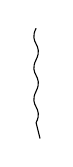
\begin{tikzpicture}
\draw (0,1.4)..controls(-.1,1.2)and(.1,1.2)..(0,1)..controls(-.1,.8)and(.1,.8)..(0,.6)..controls(-.1,.4)and(.1,.4)..(0,.2)--(.05,0);
\end{tikzpicture}}}
\margin{\figure{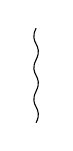
\begin{tikzpicture}
\draw (0,1.2)..controls(-.1,1)and(.1,1)..(0,.8)..controls(-.1,.6)and(.1,.6)..(0,.4)..controls(-.1,.2)and(.1,.2)..(0,0);
\end{tikzpicture}}}
\margin{\figure{\begin{tikzpicture}\draw (.12,2)--(0,2)--(0,0)--(.12,0);\end{tikzpicture}}}
\margin{\figure{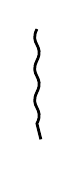
\begin{tikzpicture}
\draw[line width=1pt] (0,1.4)..controls(-.1,1.2)and(.1,1.2)..(0,1)..controls(-.1,.8)and(.1,.8)..(0,.6)..controls(-.1,.4)and(.1,.4)..(0,.2)--(.05,0);
\end{tikzpicture}}}
\margin{\figure{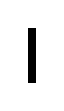
\begin{tikzpicture}\fill (0,0) rectangle(.1,.7);\end{tikzpicture}}}
\figure{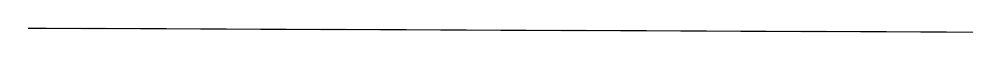
\begin{tikzpicture}\draw (0,0)--(12,-.05);\end{tikzpicture}}

\deleted{
$*$ \deleted{James September 1963}

$*$ Bott September 1963 ?

$*$ \uline{Zariski} for Dieudonné: \unsure{Give} a talk at the Colloquium of Harvard

$*$ \uline{Hilton} on the mailing list / \unsure{Prog.} II for Kuiper for myself

\deleted{copy of my talks to Baltimore}

$*$ \deleted{Paper by Eells-Kuiper.}
}
\figure{\begin{tikzpicture}
\draw (.2,2.6)--(0,2.6)--(0,1);\draw(.4,1.7)--(2.2,1.7);
\draw(.4,.7)--(2.4,.7);\draw(.4,-.8)--(2.5,-.8);\draw(0,-1.8)--(3,-1.8);
\draw(6.2,.6)--(6.3,-.8)--(6.1,-.8);
\end{tikzpicture}}
\mspage{117}

\scanpage{119}
\[
\underline{\operatorname{Ext}}^i(A,\mu_\infty)=
\left\{\begin{array}{l}0\\{}_\infty B\\0\\0\end{array}\right.
\]
\[
\underline{\underline{\operatorname{Ext}}}^i(A,\mu_\infty)\simeq H^{i-1}(K,{}_\infty B)
=\left\{\begin{array}{l}0\\H^0(K,{}_\infty B)\\H^1(K,{}_\infty B)^{\unsure{\times}}\\0\end{array}\right.
\]
\[
H^i(K,A)=\left\{\begin{array}{l}A(K)^{\unsure{\times}}\\H^1(K,A)\\\unsure{\oplus|0}\\0\\0\end{array}\right.
\]
\[
\deleted{B\qquad H^1(K,{}_\infty B)\longrightarrow H^1(K,B)\mathrel{-}0}
\]
\[
0\longrightarrow H^0(K,B)\unsure{\otimes\mathbb Q/\mathbb Z}\mathrel{-}
H^1(K,{}_\infty B)\longrightarrow H^1(K,B)\mathrel{-}0
\]
\deleted{$H^1(K,A)\longrightarrow$}
\diagram{\begin{tikzcd}[column sep=small,row sep=large]
0\arrow[r,dash]&H^0(K,{}_\infty B)\arrow[r]&DH^1(K,A)\arrow[r]\arrow[d,equal]
\arrow[dr,bend left=40]&\deleted{H^1(K,{}_\infty B)}&\\
&&H^0(K,B)&\inserted{H^0(K,B)\otimes\mathbb Q/\mathbb Z}\arrow[dl,bend right=40]&\\
&&H^1(K,{}_\infty B)\arrow[r]&DH^0(K,A)\arrow[r]\arrow[d,equal]&0\\
&&&H^1(K,B)&
\end{tikzcd}}
\figure{\begin{tikzpicture}[x=.7cm,y=.6cm]
\draw (0,4)--(12,4);\draw(.4,3.9)--(.45,1.5)..controls(.45,.9)and(.8,.8)..(1.7,.8)
--(5,.8)..controls(6,.8)and(7,.7)..(7,.3)..controls(7,-.1)and(9,0)..(12,-.5);
\end{tikzpicture}}
\[
0\mathrel{-}H^0(K,{}_\infty B)\mathrel{-}DH^1(K,A)\longrightarrow Q\mathrel{-}0
\]
\[
0\mathrel{-}N\mathrel{-}H^1(K,{}_\infty B)\mathrel{-}DH^0(K,A)\mathrel{-}0
\]
\[
\deleted{Q:\ \deleted{H^1(K,B)}\ \operatorname{Ker}\ H^0(K,B)\longrightarrow
H^0(K,B)\otimes\mathbb Q/\mathbb Z}
\]
\[
Q\subset N\qquad H^0(K,B)\longrightarrow H^0(K,B)\otimes\mathbb Q/\mathbb Z
\]
\mspage{118}

\scanpage{120}
\[
\underline{\operatorname{Ext}}^i(A,{}_n\mu)=\left\{\begin{array}{l}0\\{}_nB\\0\\0\end{array}\right.
\]
\margin{$\begin{array}{c}\mathbb Z/n\mathbb Z\\B\end{array}$}
\diagram{\begin{tikzcd}[row sep=small]
\underline{\underline{\operatorname{Ext}}}^i(A,{}_n\mu)\simeq H^{i-1}(K,{}_nB)\\[-1ex]
\unsure{\wr}\\[-1ex]
\operatorname{Ext}^{i-1}(T(A),\mathbb Z/n\mathbb Z)
\end{tikzcd}}
\[
H^i(K,{}_nB)\xrightarrow{\sim}\operatorname{Ext}^i_{k\text{-gr}}(T(A),\mathbb Z/n\mathbb Z)
\]
\diagram{\begin{tikzcd}[column sep=small,row sep=small]
H^i(K,{}_\infty B)\simeq\operatorname{Ext}^i_{k\mathrm{gr}}(&T(A)\arrow[d,leftrightarrow],&\mathbb Q/\mathbb Z)\\
&\mathcal A&H^1(K,A)
\end{tikzcd}}
\[
{}_nB(K),H^1(K,{}_nB),0\mathrel{-}\mathrel{-}\ \big|\qquad
[\text{dual de }H^1(K,{}_nA)]
\]
\figure{\begin{tikzpicture}[x=.7cm,y=.7cm]
\draw[line width=1.8pt,-stealth](0,.3)--(-.2,0)--(3,0);
\node[below]at(1.6,-.3){$V\times\deleted{\unsure{\mathbb Z}}D\mathrel{-}\text{\uline{discrète}}$};
\end{tikzpicture}}
\figure{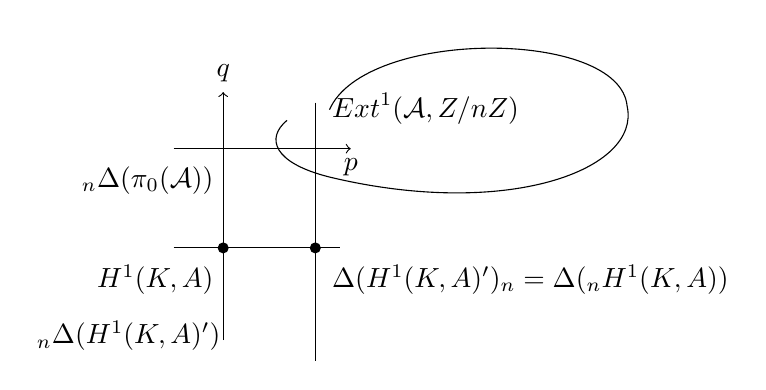
\begin{tikzpicture}[x=.9cm,y=.9cm]
\draw[->](-.7,0)--(1.8,0)node[below]{$p$};
\draw[->](0,-2.7)--(0,.8)node[above]{$q$};
\draw(1.3,.65)--(1.3,-3);\draw(-.7,-1.4)--(1.65,-1.4);
\fill(0,-1.4)circle(2pt);\fill(1.3,-1.4)circle(2pt);
\node[above right]at(1.4,.2){$\operatorname{Ext}^1(\mathcal A,\mathbb Z/n\mathbb Z)$};
\draw(1.5,.55)..controls(2,1.7)and(5.6,1.7)..(5.7,.6)..controls(5.9,-.3)and(4,-1)..(1.5,-.4)..controls(.7,-.2)and(.6,.15)..(.9,.4);
\node[left]at(0,-.45){${}_n\Delta(\pi_0(\mathcal A))$};
\node[below left]at(0,-1.5){$\deleted{\unsure{H^1(K,A)}}$};
\node[below left]at(.1,-2.3){${}_n\Delta(H^1(K,A)')$};
\node[below right]at(1.4,-1.5){$\Delta(H^1(K,A)')_n=\Delta({}_nH^1(K,A))$};
\end{tikzpicture}}
\noindent $1^\circ)$ la partie discrète de $H^1(K,A)$ est \uuline{divisible}

\noindent $2^\circ)$
\[
0\mathrel{-}\mathbb Z/n\mathbb Z\mathrel{-}\mathbb Q/\mathbb Z\overset{n}{\mathrel{-}}\mathbb Q/\mathbb Z\mathrel{-}0
\]
\noindent (i) $H^1(K,A)'$ divisible, i.e. $\Delta H^1(K,A)'$ \deleted{$\unsure{a\mathbb Z}$} \inserted{sans torsion}

\noindent (ii) $H^1(K,{}_nB)\xrightarrow{\sim}\operatorname{Ext}^1_{k\mathrm{gr}}(\mathcal A,\mathbb Z/n\mathbb Z)$
\margin{?}

\noindent (iii) $\unsure{u|n}$
\mspage{119}

\scanpage{121}
\mspage{III-42}
En outre, on sait que $H^i(X,\underline F)=0$ sauf pour un nombre fini de valeurs de $i$ (\uline{loc.cit.}) ; le nombre entier
\[
(15)\qquad\chi_A(\underline F)=\sum_{i=0}^{\infty}(-1)^i\operatorname{Long}(H^i(X,\underline F))
\]
est donc défini pour tout $\underline O_X$-module cohérent $\underline F$ ; on l'appelle la \uline{caractéristique d'Euler-Poincaré de $\underline F$} (\uline{par rapport à l'anneau A}).
\margin{si $A$ est local}
\figure{\begin{tikzpicture}[x=.6cm,y=.6cm]\draw(0,0)--(.1,1.5);\draw(.1,1.5)circle(.08);\draw(5,0)--(5.5,1.4);\draw(5.5,1.4)circle(.08);\end{tikzpicture}}
Pour $\underline F=\underline O_X$, on dit que $\chi_A(\underline O_X)$ est le \uline{genre} \deleted{\illegible{1}} \uline{arithmétique} de $X$.

\uline{Proposition 13 .- Soit} $0\to\underline{F'}\to\underline F\to\underline{F''}\to0$ \uline{une suite exacte de $\underline O_X$-modules cohérents. On a alors}
\[
(16)\qquad\chi_A(\underline F)=\chi_A(\underline{F'})+\chi_A(\underline{F''}).
\]
On a en effet, par la suite exacte de cohomologie, une suite \unsure{exacte}
\[
\begin{gathered}
0\to H^0(X,\underline{F'})\to H^0(X,\underline F)\to H^0(X,\underline{F''})\to H^1(X,\underline{F'})\to\cdots\\
\to H^r(X,\underline{F'})\to H^r(X,\underline F)\to H^r(X,\underline{F''})\to0
\end{gathered}
\]
\deleted{\illegible{1}} les modules de cohomologie d'indice $>r$ étant nuls pour $\underline F$, $\underline{F'}$ et $\underline{F''}$. Or on sait que dans une suite exacte de modules de longueur finie, ayant des 0 aux deux extrémités, la somme alternée des longueurs est nulle ; appliquant ce résultat, on trouve immédiatement (16).

\uline{Théorème 2 .-} \inserted{\uline{Soit $\underline F$ un $\underline O_X$-module cohérent}.}
(i) \deleted{\illegible{3}} \uline{La fonction} $n\to\chi_A(\underline F(n))$ \uline{est \inserted{égale à} un polynôme \inserted{en $n$}.}

(ii) \uline{Pour n assez grand, on a} $\chi_A(\underline F(n))=\operatorname{Long}\Gamma(X,\underline F(n))$ ; \uline{si} $\underline F=\widetilde M$, \deleted{\illegible{2}} (\uline{où M est un S-module gradué de type fini}), \uline{on a} $\chi_A(\underline F(n))=\operatorname{Long}(M_n)$ \uline{pour n assez grand}.

(iii) \uline{Le terme de plus haut degré de} $\chi_A(\underline F(n))$ \uline{a un coefficient} $\geq0$.
\margin{$>$}

(iv) \uline{Le degré de} $\chi_A(\underline F(n))$ \uline{est égale à la dimension du support de $\underline F$}.

Soient \deleted{$\unsure{z}$} $\xi_1,\ldots,\xi_m$ les points de $Z=\operatorname{Spec}(A)$ ; on sait que \deleted{$\unsure{Z}$} $Z$ est somme des schémas $Z_i=\operatorname{Spec}(A_i)$, \deleted{\unsure{et}} où \deleted{\unsure{les}} les $A_i$ sont les composants locaux de $A$, et l'espace de base de $Z_i$ est $\{\xi_i\}$ (I,4,1,prop.4) ; si $f:X\to Z$ est le morphisme structural, $X$ est alors somme des présché-
\margin{\unsure{Joube|doute}}
\figure{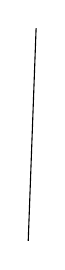
\begin{tikzpicture}\draw(0,0)--(.1,2.7);\end{tikzpicture}}
\mspage{120}

\scanpage{122}
\begin{flushright}
Corps de classes\\
et dualité\\
des \uline{Courbes Algébriques}
\end{flushright}
\mspage{121}

\scanpage{123}
\diagram{\fbox{$\begin{array}{ll}
H^i_Y(X,M)&\operatorname{Ext}^i(X,M,A)\\[1ex]
H^i(X,M)&\operatorname{Ext}^i_Y(X,M,A)\\[1ex]
H^i(U,M)&\operatorname{Ext}^i(U,M,A)
\end{array}$}}
\[
\operatorname{Ext}_{\unsure{m}}(M,A)\overset{?}{=}D(M)\qquad A
\]
\[
0\mathrel{-}M'\mathrel{-}M\mathrel{-}M''\mathrel{-}0
\]
\[
\unsure{\operatorname{Hom}}_{\unsure{m}}(M,A).
\]
\figure{\begin{tikzpicture}\draw(0,0)--(1.2,4.2);\draw(.08,0)--(1.29,4.25);\end{tikzpicture}}
\diagram{\begin{tikzcd}[row sep=small,column sep=large]
\operatorname{Ext}^i_Y(X;M,N)\arrow[d]&\bullet&\operatorname{Ext}^{1-i}(X;N,M)\\
\operatorname{Ext}^i(X;M,N)\arrow[d]&&\operatorname{Ext}^{1-i}_Y(X;N,M)\arrow[u,dash]\\
\operatorname{Ext}^i(U;M,N)&&\operatorname{Ext}^{-i}(U;N,M)\arrow[u,dash]
\end{tikzcd}}
\figure{\begin{tikzpicture}\draw(0,0)ellipse(.4cm and .6cm);\fill(.04,.07)circle(1.5pt);\end{tikzpicture}}
\[
\operatorname{Ext}^i_Y(X;F,G)\longrightarrow\operatorname{Ext}^i_Z(X;F,G)\longrightarrow\operatorname{Ext}^i_{Z-Y}(X;F,G)
\]
\diagram{\begin{tikzcd}[column sep=small,row sep=tiny]
\operatorname{Ext}^{\unsure{r-i}}(X_{/Y}-Y,G_{/\unsure{Y|Z}},F_{/\unsure{Y|Z}})&
\operatorname{Ext}^{r-i}_a(\unsure{\widehat X|X}_{/Y},\widehat G_{/Y},\widehat F_{/Y})\arrow[l,"?"']&
\operatorname{Ext}^{r-i}_a(X_{/Z};G_{/Z},F_{/Z})\arrow[l]&
\operatorname{Ext}^{r-i-1}(X_{/Z}-Y,G_{/Z},F_{/Z})\arrow[l,"?"']\\
&\unsure{U}\ ?&&
\end{tikzcd}}
\[
Y\subset Z
\]
\diagram{\begin{tikzcd}[row sep=tiny,column sep=large]
X_{/Y}\arrow[r]&X_{/Z}\\
&\cup\\[-1ex]
&Y\\[-1ex]
&\cup\\[-1ex]
&\{a\}
\end{tikzcd}}
\margin{$\unsure{1}$}
\[
\mathrel{-}\operatorname{Hom}_a(X_{/Z};G_{/Z},F_{/Z})
\]
\figure{\begin{tikzpicture}\draw(0,0)--(0,.17);\draw(.08,-.01)--(.08,.13);\end{tikzpicture}}
\mspage{122}

\scanpage{124}
\mspage{84}
\margin{n$^\circ$ 239}
THEOREME 3. - \uline{Soit} $\mathcal A$ \uline{un faisceau mou d'anneaux sur un espace} paracompact X. \uline{Pour tout recouvrement ouvert} $\mathcal U$ \uline{de} X, \uline{il existe dans} $\mathcal A$ \uline{une partition de l'unité subordonnée à} $\mathcal U$.

Notons d'abord que s'il existe une partition de l'unité $(s'_\mu)_{\mu\in M}$ subordonnée à un recouvrement ouvert $\mathcal U'=(U'_\mu)_{\mu\in M}$ \uline{plus fin} que $\mathcal U$, il existe aussi une partition de l'unité $(s_\lambda)_{\lambda\in L}$ subordonnée à $\mathcal U=(U_\lambda)_{\lambda\in L}$. En effet, par hypo thèse il existe une application $\varphi$ de M dans L telle que $U'_\mu\subset U_{\varphi(\mu)}$ pour tout $\mu\in M$. Lorsque $\lambda$ parcourt L, ceux des ensembles $M_\lambda=\varphi^{-1}(\lambda)$ non vides forment une partition de M. En prenant $s_\lambda=0$ si $M_\lambda=\varnothing$, $s_\lambda=\sum_{\mu\in M_\lambda}s'_\mu$ dans le cas contraire, il est immédiat que $(s_\lambda)$ est une partition de l'unité répondant à la question.

Comme X est paracompact, on peut appliquer la remarque précédente pour se ramener au cas où $\mathcal U=(U_\lambda)$ est un recouvrement \uline{localement fini}. Il existe un recouvrement ouvert $(V_\lambda)_{\lambda\in L}$ de X tel que $\overline V_\lambda\subset U_\lambda$ pour tout $\lambda\in L$. Soit $\unsure{\mathfrak S|\mathcal G}$ l'ensemble des couples $(J,\sigma_J)$, où J parcourt l'ensemble des parties de L, et pour chaque J, $\sigma_J=(s_\lambda)_{\lambda\in J}$ est une famille de sections au-dessus de X, telle que le support de $s_\lambda$ soit contenu dans $U_\lambda$ pour tout $\lambda\in J$ et que l'on ait $\sum_{\lambda\in J}s_\lambda(x)=1_x$ pour tout $x\in V_J=\bigcup_{\lambda\in J}V_\lambda$. L'ensemble $\unsure{\mathfrak S|\mathcal G}$ n'est pas vide, car il contient $(\varnothing,\varnothing)$ (le second terme étant la famille vide de sections de $\mathcal A$ au-dessus de X). Ordonnons $\unsure{\mathfrak S|\mathcal G}$ en posant $(J,\sigma'_J)\leq(K,\sigma''_K)$ si $J\subset K$ et si, pour tout $\lambda\in J$, $s'_\lambda=s''_\lambda$ ; cet ensemble est \uline{inductif}, comme on le vérifie immédiatement. Soit $(J,\sigma_J)$ un élément maximal de $\unsure{\mathfrak S|\mathcal G}$; il suffira de prouver que $J=L$. Supposons le contraire, et soit $\mu\in L-J$ ; montrons qu'il existe une section $s_\mu$ de $\mathcal A$ au-dessus de X, dont le support est
\mspage{123}

\scanpage{125}
\[
\operatorname{Ext}^i_Y(X,F,G)=\varinjlim_n\operatorname{Ext}^i(F/\mathcal J^nF,G)
\]
\margin{\unsure{dual}}
\diagram{\begin{tikzcd}[column sep=large,row sep=large]
\simeq\varprojlim_n\operatorname{Ext}^{r-i}_a(X;G,F/\mathcal J^nF)&
H^p_a(X,\underline{\operatorname{Ext}}^q_{\underline O_X}(G,F_{\unsure{n}}))\arrow[l,Rightarrow]\\
\varprojlim_n\operatorname{Ext}^{r-i}_a(\widehat X,\widehat G,\widehat F_n)\arrow[u,"\sim"]&
H^p_a(\widehat X,\underline{\operatorname{Ext}}^q_{\underline O_X}(\widehat G,\widehat F_{\unsure{n}}))\arrow[l,Rightarrow]\\
\operatorname{Ext}^{r-i}_a(\widehat X,\unsure{\widehat G|\widehat C},\widehat F_{\unsure{n}})\arrow[u]&
\end{tikzcd}}
\margin{$\lim$}
\[
\operatorname{Ext}^i_{Y-Z}(X,F,G)=\varinjlim_n\operatorname{Ext}^i(X-Z,F/\mathcal J^nF,G)
\]
\noindent \unsure{dual}
\[
\simeq\varprojlim\qquad\varprojlim\operatorname{Ext}^{r-i}(\widehat X,\unsure{\widehat G|\widehat C},\widehat F)
\]
\[
H^i(X-Z,F
\]
\margin{$Z\subset Y$}
\noindent $\mathfrak X$ \unsure{schéma} formel
\diagram{\begin{tikzcd}[column sep=small,row sep=large]
T\arrow[r,phantom,"\subset" description]&Z\arrow[r,phantom,"\subset" description]\arrow[rr,bend right=20]&\mathfrak X&\text{partie \unsure{fermée}}\\
&&\mathfrak X_{/Z}\arrow[u]&\text{complété formel le long de }Z
\end{tikzcd}}
\[
H^i_T(\mathfrak X,\mathfrak F)\longrightarrow H^i_T(\mathfrak X,\mathfrak F_{/Z})\overset{?}{\mathrel{-}}H^i(\mathfrak X
\]
\mspage{124}

\scanpage{126}
\mspage{78}
\margin{n$^\circ$ 239}
3. \uline{Faisceaux mous}.

Si X est un espace paracompact, $\mathcal F$ un faisceau de base X, Y une partie fermée de X, on a vu (th.1) que toute section de $\mathcal F$. au-dessus de Y se prolonge en une section au-dessus d'un \uline{voisinage} de Y, mais elle ne se prolonge pas nécessairement en une section au-dessus de X \uline{tout entier}.

Une raison suffisante est qu'il peut n'exister aucune section au-dessus de X tout entier (\S\ 1, exerc.1). Un autre exemple est le suivant : soient X un espace connexe séparé et paracompact, G un ensemble ayant au moins deux éléments distincts, $\mathcal F$ le faisceau constant $X\times G$, a et b deux points distincts de X, s une section au-dessus de $\{a,b\}$ telle que $s(a)=(a,\alpha)$, $s(b)=(b,\beta)$ avec $\alpha\neq\beta$ ; cette section ne peut être prolongée au-dessus de X tout entier (cf.\S\ 1, n$^\circ$ 2, \uline{Exemple}).

On va voir que, si X est paracompact, la possibilité de prolonger toute section au-dessus d'une partie fermée de X à X tout entier est une propriété \uline{locale} du faisceau $\mathcal F$.

DEFINITION 1. - \uline{Soit} X \uline{un espace localement paracompact}. \uline{On dit qu'un faisceau} $\mathcal F$ \uline{de base} X \uline{est mou s'il existe une base} $\phi$ \uline{de la topologie de} X, \uline{telle que pour tout} $U\in\phi$, $\overline U$ \uline{soit paracompact}, \uline{et, pour chaque} $U\in\phi$, \uline{un ensemble} $\psi(U)$ \uline{de parties fermées de} X \uline{contenues dans} U, \uline{satisfaisant aux conditions suivantes}. :

$(\mathrm{FM}_{\mathrm I})$ \uline{Pour tout} $U\in\phi$, \uline{toute partie fermée} M \uline{de} X, \uline{contenue dans} U, \uline{et tout voisinage} V \uline{de} M, \uline{il existe} $F\in\psi(U)$ \uline{telle que} $M\subset F\subset V$.

$(\mathrm{FM}_{\mathrm{II}})$ \uline{Quels que soient} $U\in\phi$, $F\in\psi(U)$ \uline{et la section} s \uline{de} $\mathcal F$ \uline{au-dessus de} F, \uline{il existe une section de} $\mathcal F$ \uline{au-dessus de} U \uline{prolongeant} s.
\mspage{125}

\scanpage{128}
\deleted{\unsure{Schémas}}

$C$ courbe algébrique [complète non singulière sur $k$]

\deleted{\illegible{1}} On suppose définie la notion de $C$-groupes [= faisceaux de Weil sur les préschémas de \deleted{\unsure{petit}} type fini sur $C$, pour la descente fid plate\ldots]. \deleted{\unsure{Ils}} Les $C$-groupes forment une catégorie abélienne avec assez d'injectifs, d'où des Ext (globaux et locaux), des $H^i(C,G)$ \inserted{$\simeq\operatorname{Ext}^i(C;\mathbb Z,G)$}, etc.

Sur $k$, on a les $k$-groupes [définis comme les $C$-groupes ? Cela est-il équivalent aux foncteurs de Weil \inserted{-schémas} sur les \deleted{\unsure{les}} $k$-ensembles algébriques ?]

On a un foncteur \deleted{$\unsure{f_*}$}
\[
f_*:\operatorname{Gr}_C\mathrel{-}\operatorname{Gr}_k\mathrel{-}\operatorname{QuGr}_k
\]
[image directe par $f:C\mathrel{-}\operatorname{Spec}k$] qui est exact à g., \deleted{\unsure{donc}} et transforme injectifs en injectifs, d'où des foncteurs dérivés
\[
\underline H^i_f(G)=\deleted{\unsure{Rf(E}}\ H^i(Rf_*)(G)
\]
[si $G$ est un complexe \unsure{borné} \unsure{à} \unsure{g.} --- \unsure{nous admettrons} que $f_*$ \uline{est de dim \unsure{ch.} finie}] On définit de $\unsure{=}$
\[
\underline{\operatorname{Ext}}^i_f(F,G)=H^i(\underline E^{\unsure{\bullet}}_f(F,G))
=H^i((R\underline{\operatorname{Hom}}_f(F,-))(G))
\]
D'où comme d'habitude des suites spectrales
\[
\deleted{H^{\unsure{i}}_f}\quad\operatorname{Ext}^{\unsure{*}}(C;F,G)
\Longleftarrow H^p(\unsure{K|X};\underline{\operatorname{Ext}}^q(F,G))
\]
en particulier
\[
H^{\unsure{*}}(C,G)\Longleftarrow H^p(k;\underline H^q_f(G))
\]
\mspage{127}

\scanpage{129}
\deleted{
\deleted{Proposition}
\margin{passer au N$^\circ$ \unsure{précédent}}
\figure{\begin{tikzpicture}\draw[->](0,0)..controls(-.8,1)and(-.8,2)..(.6,2.8);\draw(1,2.6)--(1.5,1.8)--(2.8,2.6);\draw(1.5,1.8)circle(.06);\end{tikzpicture}}

(i) Si $A=k[t_{\unsure{1|0}},-,t_n]_{\mathfrak m}$, $\mathfrak m$ maximal, $k$ un corps alors \deleted{$\dim A=n\quad A$ est de dim} \inserted{$A$ est \uline{régulier}, de dim $n$} $\dim A=n$
\margin{\deleted{$A[t_1--t_n]$}}

\uline{Dem.} Par \unsure{chgt} de base, on est \unsure{ramené} au cas où $k(\mathfrak m)=k$, on a alors une \deleted{\unsure{régulière de}} \inserted{$A$-suite} \deleted{paramètres} de $n$ éléments engendrant l'idéal maximal $\mathfrak m$

\margin{\deleted{\unsure{(ii)}} \uline{Cor}}
$A$ anneau \inserted{local} noeth. Alors pour tt idéal maximal $M$ de $B=A[t_1-t_n]$ induisant $M\cap A=\mathfrak m$, on a
\[
\dim B_M=\dim A+n
\]
\uline{Cor} si $A$ \unsure{anneau local} noeth, $\dim A[t_1,-,t_n]=\dim A+n$

\uline{Cor} Utilisons la formule des dimensions dans le cas des algèbres de type fini sur $k$. [\unsure{résulte du} lemme de normalisation] on trouve, si $M$ induit $\mathfrak m$
\[
\dim B_M=\dim A+\underbrace{n-\deg\operatorname{tr}\ k(M)/k(\mathfrak m)}_{\nu=\dim[ B_M\otimes_A k=k[t_1,-t_n]_M ]}
\]
\deleted{\uline{Cor} $A$ anneau noeth. Alors $\dim A[t_1,-t_n]=\dim A+n$}

\deleted{(ii) Si $A=k[t_1,-t_n]_{\mathfrak m}$, $\mathfrak m$ maximal, $k$ un corps, \unsure{Alors} $A$ \unsure{est}}
\figure{\begin{tikzpicture}[x=.65cm,y=.65cm]
\draw(0,3.6)--(.1,1.8)..controls(1.8,1.7)and(4.5,1.8)..(5.8,2.3)--(6,3.6);
\draw(3.4,3.2)..controls(3.3,2.2)and(4,2)..(4.7,2.6)..controls(4.9,2.8)and(5,2.2)..(5.4,2.4);
\draw(1.7,3.5)--(1.6,2.4)..controls(1.6,1.8)and(2.2,3.1)..(2.5,2.5);
\draw(0,1.8)--(.4,.7)--(3.7,.95);\draw(.2,.7)..controls(.5,2.2)and(.5,-.1)..(1.1,1.5)..controls(1.4,.8)and(1.7,.8)..(2,1.4)..controls(2.2,.7)and(2.8,.6)..(3.5,1.1);
\node at(2.8,.9){$\unsure{A\Gamma}$};
\draw(2.7,2.2)..controls(3.2,1.2)and(3.2,.1)..(3.9,-.6);
\end{tikzpicture}}
\uline{Dem.} \deleted{\unsure{Prof}}
\[
\left\{\begin{array}{l}
\operatorname{prof}B_M=\operatorname{prof}A+\nu\\[1ex]
\operatorname{coprof}\unsure{B_M|\Phi_M}=\operatorname{coprof}A-
\end{array}\right.
\]

\uline{Cor.} $X=Y[t_1-t_n]$, $Y$ loc. noeth. \unsure{soit $x\in X$}, $y\in Y$. Soit P l'une des propriétés\ldots\ldots. Alors $X$ est P \unsure{en $x$} si $Y$ est \unsure{''|``}\unsure{en $y$}.
\unsure{(Montrer} \unsure{pour} \unsure{certaines} propriétés).
\figure{\begin{tikzpicture}\draw(0,0)--(0,2.2);\end{tikzpicture}}
}
\mspage{128}

\scanpage{130}
\deleted{
Soit un elt $\unsure{f|\varphi}\in\operatorname{Ext}^i(C;G,S\unsure{\sigma|\tau})$, i.e. un hom de degré $i$ $G\mathrel{-}S\unsure{\sigma|\tau}$, d'où un hom de degré $i$ $Rf_*G\mathrel{-}Rf_*S\unsure{\sigma|\tau}$, donc il reste à définir un hom de degré $0$
\[
Rf_*S\unsure{\sigma|\tau}=Rf_*(\unsure{\sigma|\tau}\otimes\mu_n(1))\longrightarrow\unsure{\sigma|\tau}
\]
\[
R^{\unsure{i}}
\]
i.e. un élément de
\[
\operatorname{Ext}^2(k,Rf_*(\unsure{\sigma|\tau}\otimes\mu_n),\unsure{\sigma|\tau})\mathrel{-}\quad---
\]
}
On a un hom \unsure{évident}
\[
\underline E_f(G,S\unsure{\sigma|\tau})\mathrel{-}E_f(Rf_*G,Rf_*S\unsure{\sigma|\tau})
\]
et si nous définissons un élément
\[
\gamma\in\deleted{\unsure{\operatorname{Ext}^0}}\inserted{\operatorname{Hom}^0}(Rf_*S\unsure{\sigma|\tau},\unsure{\sigma|\tau})
\]
nous en déduisons un \deleted{élément} hom
\[
E_f(Rf_*G,Rf_*S\unsure{\sigma|\tau})\mathrel{-}E_f(Rf_*G,\unsure{\sigma|\tau})
\]
et en composant, on trouve l'hom voulu
\[
E_f(G,S\unsure{\sigma|\tau})\longrightarrow E_f(Rf_*G,\unsure{\sigma|\tau})
\]
Ceci dit, le th. de dualité s'énonce

\uline{Th.} (i) Si $G$ est \inserted{un \deleted{\unsure{proalgébrique}} faisceau de Weil} fini [plus gén les $\unsure{H^i(G)}$ sont \deleted{\unsure{tous finis}}], \deleted{alors} plus gén est affine, et sans composantes abéliennes, alors
\[
E_f(G,S\unsure{\sigma|\tau})\xrightarrow{\sim}E(Rf_*G,\unsure{\sigma|\tau})
\]
\margin{\unsure{préciser}}
\figure{\begin{tikzpicture}\draw(0,0)--(0,1.2);\end{tikzpicture}}
(ii) Si $G$ est \inserted{\figure{\begin{tikzpicture}[baseline=(t.base)]\node[ellipse,draw,inner xsep=6pt,inner ysep=1pt](t){de type fini};\end{tikzpicture}}} sans composantes abéliennes, alors $E_f(G,S\unsure{\sigma|\tau})\longrightarrow E(Rf_*G,\unsure{\sigma|\tau})$ est un isom mod $\theta$ [i.e. \unsure{les} $\underline E$ dans $\mathbb Q/\mathbb Z$ \deleted{\unsure{est un}} \unsure{se transforme} en un isom\ldots].
\mspage{129}

\scanpage{131}
$\underline{\overline{\mathrm V}}$\quad\deleted{$\unsure{\mathrm{IV}|\mathrm{VI}}$}
\begin{flushright}
\deleted{\uuline{Schémas de Hilbert, de Picard}}

\deleted{(sans théorie des\\
relations \unsure{intimes} avec les\\
groupes fondamentaux)}
\end{flushright}
\mspage{130}

\scanpage{132}
On a une suite exacte de $C$-groupes
\diagram{\begin{tikzcd}
0 \arrow[r] & \mu_n \arrow[r] & G_m \arrow[r,"n"] & G_m \arrow[r,dash] & 0
\end{tikzcd}}
d'où
\diagram{\begin{tikzcd}
H^1(C,G_m) \arrow[r,"n"] & H^1(C,G_m) \arrow[r,dash] & H^2(C,\mu_n) \arrow[r] & H^2(C,G_m)
\end{tikzcd}}
[N.B. On a $\underline H^i_f(G_m)=0$ pour $i\geq2$, \inserted{$\underline H^0_f(G_m)\simeq G_m$,} d'où une suite exacte\unsure{\ldots}]
\diagram{\begin{tikzcd}[column sep=small]
0 \arrow[r] & H^1(k,G_m) \arrow[r] \arrow[d,equal] & H^1(C,G_m) \arrow[r] & H^0(k,\underline H^1_f(G_m)) \arrow[r] \arrow[d,equal] & H^2(k,G_m) \arrow[d,equal] \\
& 0 & & \operatorname{Pic}(C/k) & \operatorname{Br}(k) \\
& \unsure{\text{th. 90}} & & &
\end{tikzcd}}
Ainsi, $H^1(C,G_m)\subset\operatorname{Pic} C$.

$\unsure{\sigma|\tau}$ groupe \inserted{fini} \deleted{\unsure{ab}} \unsure{étale} sur $k$,
définit un groupe \deleted{$\unsure{\sigma|\tau}\otimes\mu_n$ sur $k$ de} $D(\Delta\unsure{\sigma|\tau})$ de type multiplicatif [isomorphe à $\unsure{\sigma|\tau}\otimes\mu_n$ si $n\unsure{\sigma|\tau}=0$].

Posons $S\unsure{\sigma|\tau}=(D\Delta\unsure{\sigma|\tau})(2)$

On va définir un \deleted{hom} accouplement
\[
\text{a)}\qquad \operatorname{Ext}^i(C;G,S\unsure{\sigma|\tau})\longrightarrow
\operatorname{Ext}^{i\deleted{\unsure{-2}}}(k;Rf_*G,\unsure{\sigma|\tau})
\]
associé à un hom
\[
\text{b)}\qquad \text{\textcircled{$*$}}\qquad
\underline E_f(G,S\unsure{\sigma|\tau})\longrightarrow\underline E_k(Rf_*G,\unsure{\sigma|\tau})
\]
[évidemment bifonctoriel en $G,\unsure{\sigma|\tau}\ldots$], qui définit aussi un hom
\[
\underline{\operatorname{Ext}}^i_f(G,S\unsure{\sigma|\tau})\longrightarrow
\underline{\operatorname{Ext}}^i_k(Rf_*G,\unsure{\sigma|\tau})
\]
c)
\mspage{131}

\scanpage{133}
\margin{provient du \uline{complexe \unsure{idélique}} $J$ par \unsure{multiplication} par $n$}
\figure{\begin{tikzpicture}[x=1cm,y=1cm]
\draw (0.25,3) .. controls (0,2.8) and (0,2.5) .. (0,1.7) .. controls (0,1.55) and (-0.18,1.5) .. (-0.18,1.5) .. controls (0,1.45) and (0,1.3) .. (0,1.1) .. controls (0,0.5) and (0,0.1) .. (0.25,0);
\end{tikzpicture}}
\diagram{\begin{array}{c|c}
\mu_n,\quad(n,p)=1 & \mathbb Z/n\mathbb Z\qquad(n,p)=1\\[5pt]
\mu_n,\quad {}_nJ,\quad\mathbb Z/n\mathbb Z & \mathbb Z/n\mathbb Z=\mu_n\otimes\mu_n^\vee,\quad {}_nJ\otimes\mu_n^\vee,\quad\mu_n^\vee\\[8pt]\hline
\mu_p & \mathbb Z/p\mathbb Z\\[5pt]
\mu_p,\quad {}_pJ,\quad\mathbb Z/p\mathbb Z & \mathbb Z/p\mathbb Z,\quad {}_{(1-F)}H^1(C,\underline O_C)^{\unsure{F}},\quad H^1(C,\underline O_C)_{(1-F)}=0\\[8pt]\hline
\alpha_p & \alpha_p\\[5pt]
\alpha_p,\quad {}_FH^1(C,\underline O_C),\quad H^1(C,\underline O_C)_F & \text{''}\\[8pt]\hline\hline
G_m & \mathbb Z\\[5pt]
\bigl[G_m,\quad\underline{\operatorname{Pic}}^{\unsure{0|\bullet}}_{C/k},\quad0, & \mathbb Z,\quad0,\quad H^1(C,\mathbb Q/\mathbb Z)=\operatorname{Hom}(T(J),\mathbb Q/\mathbb Z),\quad H^2(C,\mathbb Q/\mathbb Z)\simeq\underset{(n,p)=1}{\varinjlim}\mu_n^\vee,\quad0,\bigr]\
\end{array}}
\margin{\unsure{autodualité} des \unsure{S.} \unsure{gr. d'ordre fini} de la \deleted{\unsure{Jacobienne}}}
\margin{$\Delta({}_pJ)\simeq H^1(C,\underline O_C)^F$\par
$\phantom{\Delta({}_pJ)}\qquad\Vert$\par
$\phantom{\Delta({}_pJ)}\quad(H^1(C,\mathbb Z/p\mathbb Z))$\par
i.e. $\pi_1(C)\otimes\mathbb Z/p\mathbb Z\simeq{}_pJ$\par
[autodualité de la Jacobienne \unsure{pour} $\unsure{V,F|p}$]}
[provient du \uline{complexe adélique} $A$ par application du \deleted{\unsure{p}} \inserted{Frobenius}]
\margin{Dualité \unsure{élémentaire} de $H^1(C,\underline O_C)_F$ et ${}_FH^1(C,\underline O_C)$ provient de l'autodual. d'ordre infinitésimal de la Jacobienne, \unsure{le plus gd sous-groupe de|du plus gd sous-groupe de} $A$ (\unsure{ou} ${}_pA$) isomorphe à un $\alpha_p^n$, est dual au \unsure{plus gd quotient} de ${}_pA$ ayant la $\unsure{=}$ propriété, cette dualité provenant d'une dualité des algèbres de Lie correspondantes.}

Pour $G=G_m$, le th. de dualité s'écrit \deleted{\unsure{pour tout groupe}}
\[
H^*(C,\unsure{\sigma|\tau})\simeq
\uuline{\operatorname{Ext}}^*\bigl(\underbrace{Rf_*(G_m)}_{\substack{\text{complexe}\\\text{\unsure{idélique}}\ \unsure{J}}}(-1),\unsure{\sigma|\tau}\bigr)
\Longleftarrow\uuline{\operatorname{Ext}}^{\unsure{p+q}}(R^{-q}f_*(G_m),\unsure{\sigma|\tau})
\]
et on se ramène au cas \uline{géométrique}, et $\unsure{\sigma|\tau}=\mathbb Q/\mathbb Z$.
\[
H^*(C,\mathbb Q/\mathbb Z)\simeq\uuline{\operatorname{Ext}}^*(Rf_*(G_m)(1),\unsure{\sigma|\tau})
\Longleftarrow\uuline{\operatorname{Ext}}^{\unsure{i-j}}(R^{-j}f_*(G_m),\mathbb Q/\mathbb Z).
\]
et on calcule :
\[
H^0(C,\mathbb Q/\mathbb Z)\simeq\mathbb Q/\mathbb Z,\qquad
H^1(C,\mathbb Q/\mathbb Z)\simeq\operatorname{Ext}^1(J^{\unsure{0|\bullet}},\mathbb Q/\mathbb Z),\qquad
H^2(C,\mathbb Q/\mathbb Z)\simeq\varinjlim\mu_n^\vee
\]
\inserted{$\operatorname{Ext}^1(J^0,\mathbb Q/\mathbb Z),\quad\Vert$}
\margin{autodualité de la Jacobienne}
\figure{\begin{tikzpicture}[x=1cm,y=1cm]
\draw[<-] (0,0) -- (2.3,0.1);
\draw (2.4,0.2) .. controls (2.6,0.7) and (3.2,0.8) .. (3.6,1.1);
\draw (-3,-0.4) -- (7,-0.25);
\end{tikzpicture}}
\mspage{132}

\scanpage{134}
\deleted{$\overline{\underline{\mathrm V}}$}
\deleted{\uline{Fidèle platitude}\par
\uline{Descente} fid. plate\par
Applications}
\mspage{133}

\scanpage{135}
Ci-dessus, on a \unsure{regardé|supposé} les coefficients \unsure{simples} \inserted{\unsure{finis}}, \uline{provenant de $k$}.

Regardons le cas des faisceaux de Weil \uline{concentrés} en un point $x\in C$. Alors \deleted{$\unsure{T(G)}\simeq$} [cas géom]
\[
T(G)\simeq G_x\quad\text{``considéré comme groupe algébrique sur $k$''}
\]
On doit prouver
\[
\operatorname{Ext}^i(C;\unsure{G_x|G},\deleted{\unsure{S}}\unsure{\sigma|\tau}\otimes\mu_n)\simeq
\operatorname{Ext}^{i-2}(k;G_x,\unsure{\sigma|\tau})
\]
Il est sans doute vrai que le $\operatorname{Ext}^i$ écrit est aussi le $\operatorname{Ext}^i$ \deleted{\uline{local}} fait \unsure{sur} le \unsure{hensélisé} de $\underline O_{C,x}\ldots$
\inserted{si $G=G_Y$ (où $Y=\{x\}$),}
\margin{$Y$ \unsure{partie fermée} finie de $C$}
\figure{\begin{tikzpicture}\draw[rotate=40] (0,0) ellipse (1.8 and .7);\end{tikzpicture}}

Par la suite exacte des $\operatorname{Ext}$, on est ramené à \unsure{obtenir}
\deleted{$\operatorname{Ext}^*(C,G,\unsure{\sigma|\tau}\otimes\mu_n)\Longleftarrow H^p(C,\underline{\operatorname{Ext}}^q(G,\unsure{\sigma|\tau}\otimes\mu_n))$}
le th. de dualité, \deleted{\unsure{pour}} pour les \deleted{\unsure{G}} $i_!(F)$, i.e. : vérifions
\margin{$i:U\longrightarrow C$ est l'imm. \unsure{compl.} ($U=C-Y$)}
\figure{\begin{tikzpicture}[x=1cm,y=1cm]
\draw (-2,0) .. controls (-.8,.5) and (.8,-.5) .. (2,.2);
\draw (1.2,.2) .. controls (1,-.6) and (1.4,-1) .. (1.5,-.4) .. controls (1.6,-1.2) and (2,-1) .. (2.4,-.8);
\draw (1.1,-1) -- (2.6,-.9);
\end{tikzpicture}}
\[
\operatorname{Ext}^i(U;F,S\unsure{\sigma|\tau})\simeq
\operatorname{Ext}^{i}_{\unsure{\varphi|k}}(k;R\unsure{f_*}(\overset{\inserted{F_U}}{\overbrace{i_!F}}),\unsure{\sigma|\tau})
\]
où $\varphi_U:U\text{---}\operatorname{Spec}(k)$ est induit par $f\ldots$

\deleted{($F$ fini plat sur $U$) \unsure{premier à $p$}}

\unsure{\ensuremath{\omega})|a)} \deleted{$\unsure{F}$ \unsure{pour}} On est ramené à prouver que
\[
\boxed{H^{\unsure{i}}(U;\widehat F)\simeq\operatorname{Ext}^{i-2}(Rf_*(\deleted{\unsure{G}}F_U)),\mathbb Q/\mathbb Z)}
\]
\deleted{N.B. \unsure{bien distinguer}}\par
\deleted{\unsure{les groupes}}
\figure{\begin{tikzpicture}[x=1cm,y=1cm]
\draw (0,.3) .. controls (-.3,.9) and (-.8,.2) .. (0,.1) .. controls (.4,-.3) and (.8,.2) .. (.8,.8) .. controls (.9,-.5) and (1.3,.2) .. (1.5,.5) .. controls (1.6,.1) and (2,.1) .. (2.2,.5) .. controls (2.2,0) and (2.7,0) .. (3,.4) .. controls (3,-.2) and (3.5,0) .. (3.6,.5);
\draw (-.5,0) -- (3.3,.05);
\end{tikzpicture}}
Ce qui définit une suite exacte (\unsure{déduite} de
$\unsure{0}\longrightarrow F_U\longrightarrow F\longrightarrow F_Y\longrightarrow0$
\deleted{$\operatorname{Ext}^{\unsure{i-2}}\longleftarrow$}
\diagram{\begin{tikzcd}[column sep=small]
\cdots & H^i(U;\widehat F) \arrow[l] & \operatorname{Ext}^{i-2}(Rf_*(F_{\unsure{Y}}),\mathbb Q/\mathbb Z) \arrow[l] & \operatorname{Ext}^{i-2}(Rf_*F_{\unsure{\cdot}},\mathbb Q/\mathbb Z) \arrow[l] & {}\arrow[l]
\end{tikzcd}}
on le vérifie par un calcul facile \deleted{\unsure{essentiel}}
(\unsure{n'utilisant} que les résultats de dualité déjà vérifiés\ldots) dans le cas où $F=\mu_n$ d'où $\widehat F=\mathbb Z/n\mathbb Z$,
($n$ \deleted{\unsure{quelconque}} \inserted{premier à $p\ldots$}), en \unsure{invoquant}, \deleted{\unsure{et ensuite}} [d'où \unsure{aussi},
\mspage{134}

\scanpage{136}
$F=i_*(G)$
\[
\left\{\begin{aligned}
H^0_x(F)&=H^1_x(F)=0\\
H^2_x(F)&=H^1(K,F)
\end{aligned}\right.
\]
\[
\uuline{\operatorname{Ext}}^i(H^1(K,F),\mathbb Q/\mathbb Z)\simeq
\operatorname{Ext}^i(S,i_{\unsure{!|*}}G,\deleted{\unsure{S\sigma}},{}_\infty G_m)
\]
\[
\operatorname{Ext}^{\unsure{i}}
\]
\diagram{\begin{tikzcd}
H^i_x(F)\arrow[r]&H^i(X,F)\arrow[r]&H^i(U,F)
\end{tikzcd}}
\[
i\qquad\deleted{\operatorname{Ext}^{\unsure{j}}}\qquad\longleftarrow H^j(U,\widehat F)
\]
$F$
\diagram{\begin{tikzcd}
\underline H_x(F)\arrow[r]&\underline H_X(F)\arrow[r]&\underline H_U(F)\arrow[ll,bend left=35]
\end{tikzcd}}
\figure{\begin{tikzpicture}\draw(0,.15)--(.13,0)--(.45,.4);\end{tikzpicture}}
triangle exact de complexes de $k$-groupes

Prenant les \unsure{duals} dans $\mathbb Q/\mathbb Z$
\diagram{\begin{tikzcd}
\unsure{E|\operatorname{Ext}}(\unsure{X};F,\deleted{\unsure{\infty}}\mu_\infty)\arrow[rr,bend right=35]&E_x(X;F,\mu_\infty)\arrow[l]\arrow[l,bend left=35,"\unsure{2|?}"']&E(U;F,\mu_\infty)\arrow[l]
\end{tikzcd}}
\figure{\begin{tikzpicture}[x=1cm,y=1cm]\draw(0,0)--(11,.35);\end{tikzpicture}}
\margin{?}
\diagram{\begin{tikzcd}[column sep=small,row sep=large]
E(U;F,\mu_\infty)^n\arrow[dd,bend right=35,"\partial"']&\simeq&E(k,\underline H_U(F),\mathbb Q/\mathbb Z)^{n-1}\arrow[d,"\partial"]\\
E(X;F,\mu_\infty)^n\arrow[u,"\rho"']&\simeq&E(k,\underline H_x(F),\mathbb Q/\mathbb Z)^{n-2}\arrow[d,"i"]\\
E_x(X;F,\mu_\infty)^n\arrow[u,"i"']&\simeq&E(k,\underline H_X(F),\mathbb Q/\mathbb Z)^{n-2}\arrow[uu,bend left=35,"\rho"]
\end{tikzcd}}
\diagram{\begin{array}{ll}
E_U(X;F,\mu_\infty)^i&E(k,\underline H_U(F),\mathbb Q/\mathbb Z)^{i-1}\unsure{\simeq}\\[5pt]
\unsure{E_{\widehat X}|\widehat E_X}(X;F,\mu_\infty)&E(k,\underline H_x(F),\mathbb Q/\mathbb Z)\\[5pt]
\widehat E_x(X;F,\mu_\infty)^i&E(k,\underline H_x(F),\mathbb Q/\mathbb Z)^{i-2}
\end{array}}
\figure{\begin{tikzpicture}[x=1cm,y=1cm]
\draw(1,5.1)..controls(-.2,5.1)and(-.2,5)..(-.2,4.3)--(-.2,.2)..controls(-.2,-.2)and(.7,-.2)..(1.3,-.2)--(8.6,-.3);
\draw(.6,4.7)..controls(.4,4.5)and(.5,4)..(.3,3.8)..controls(.5,3.6)and(.4,3)..(.6,2.9);
\end{tikzpicture}}
\margin{\[
\begin{gathered}
E(U;F,\mu_\infty)^n\simeq E(X;F_U,\mu_\infty)^n\\
\rotatebox{90}{$\simeq$}\\
E(k,\underline H_x(F_U),\mathbb Q/\mathbb Z)^{\unsure{n-2}}\\
\rotatebox{90}{$\simeq$}\,!\\
E(k,\underline H_U(F),\mathbb Q/\mathbb Z)^{n-1}
\end{gathered}
\]
\[
\left\{\begin{gathered}
\underline H^m_x(F_x)^{\deleted{\unsure{m}}}\simeq\underline H^m_x(F)^{\deleted{\unsure{m}}}\\
\boxed{\underline H^m_U(F)\simeq\underline H^{m+1}_{\unsure{x|X}}(F_U)}
\end{gathered}\right\}\unsure{!!}
\]
\[
\begin{gathered}
E_x(X;F,\mu_\infty)^n\simeq E(X;F_x,\mu_\infty)^n\\
\rotatebox{90}{$\simeq$}\\
E(k,\underline H_x(F_x),\mathbb Q/\mathbb Z)^{\unsure{n-2}}\\
\rotatebox{90}{$\simeq$}\\
E(k,\underline H_X(F),\mathbb Q/\mathbb Z)^{\unsure{n-2}}
\end{gathered}
\]}
\figure{\begin{tikzpicture}[x=1cm,y=1cm]\draw(0,0)--(.1,3.5);\draw(.1,4.2)--(0,7.4);\end{tikzpicture}}
\mspage{135}

\scanpage{137}
\begin{center}- 37 -\end{center}
\margin{n°338}
\uline{l'homomorphisme} $x\longrightarrow1\otimes x$ \uline{de} $F$ \uline{dans} $B\otimes_A F$ \uline{est injectif} ;

(iv) \uline{le} $A$-\uline{module à droite} $B$ \uline{est plat, et, pour tout idéal à gauche} $\underline a$ \uline{de} $A$ \uline{on a} $h^{-1}(B\underline a)=\underline a$.

(v) \uline{le} $A$-\uline{module à droite} $B$ \uline{est plat, et, pour tout idéal à gauche maximal} $\underline m$ \uline{de} $A$, \uline{il existe un idéal à gauche maximal} $\underline{m'}$ \uline{de} $B$ \uline{tel que} $h^{-1}(\underline{m'})=\underline m$.
\margin{$\unsure{\operatorname{Spec}|\operatorname{Spm}}(B)\longrightarrow\unsure{\operatorname{Spec}|\operatorname{Spm}}(A)$ surjectif}
\figure{\begin{tikzpicture}\draw(0,0)--(.15,1.3);\end{tikzpicture}}

En effet, d'après le lemme, (i) implique chacune des propriétés (iii), (iv), (v). D'autre part, si (v) est vérifiée, on a $B\underline m\ne B$ pour tout idéal à gauche maximal $\underline m$ de $A$, et $B$ est fidèlement plat sur $A$ par définition.

Nous allons maintenant prouver que $(i)\Longrightarrow(iii)\Longrightarrow(iv)\Longrightarrow(ii)\Longrightarrow(i)$, ce qui achèvera la démonstration. On a déjà vu que (i) implique (iii). D'autre part (iii) implique (iv) en prenant $F=A/\underline a$. Si (iv) est vérifié, on voit, en prenant $\underline a=(0)$, que $h$ est injectif, et on a la suite exacte
\diagram{\begin{tikzcd}
0\arrow[r]&A\arrow[r,"h"]&B\arrow[r]&B\,h(A)\arrow[r]&0\,;
\end{tikzcd}}
cette suite vérifie la condition c) de la prop.3 du § 2 (cf. la remarque suivant cette proposition) ; d'après ladite proposition, il s'ensuit que $B/h(A)$ est plat, d'où (ii). Enfin, si (ii) est vérifiée, la prop. 3 appliquée à la suite exacte $0\longrightarrow A\xrightarrow{h}B\longrightarrow B/h(A)\longrightarrow0$ montre que $B$ est fidèlement plat. CQFD.

Dans les conditions de la prop.8, identifions $A$ à un \uline{sous-anneau} de $B$ au moyen de $h$. La relation (iv) s'écrit alors $A\cap B\underline a=\underline a$ pour tout idéal à gauche $\underline a$ de $A$. D'autre part, si $F$ est un $A$-module à gauche, on identifie $F$ à son image dans $B\otimes_A F$ par l'application $x\longrightarrow1\otimes x$ ; si $X$ est un sous-groupe additif de $F$, on note alors $BX$ le sous-$B$-module à gauche de $B\otimes_A F$ engendré par $X$. Avec ces notations on a :

PROPOSITION 9.- \uline{Soient} $B$ \uline{un anneau et} $A$ \uline{un sous-anneau de} $B$ \uline{tels que} $B$ \uline{soit}
\mspage{136}

\scanpage{138}
\margin{$\underline H^i_{\unsure{S|C}/k}(F)$\par $H$}
\diagram{\begin{tikzcd}[column sep=huge,row sep=large]
\underline H^{i-1}_{S/k}(G)\arrow[d,dash]&\underline H^{\overset{\inserted{3-i}}{\overbrace{2-(i-1)}}}_{Y/k}(S,\widehat{\unsure{G|C}})\arrow[d]\\
\underline H^{i-1}_{U/k}(\deleted{\unsure{G}}G)\arrow[d]&\deleted{\operatorname{Ext}}\inserted{\unsure{\underline H}}^{\overset{\inserted{2-i}}{\overbrace{1-(i-1)}}}_{U/k}(\widehat G)\\
\underline H^i_{Y/k}(S,G)\arrow[d]&\deleted{\operatorname{Ext}}\inserted{\unsure{\underline H}}^{2-i}_{S/k}(\widehat G)\arrow[u,leftrightarrow,line width=1.5pt]\\
\underline H^i_{S/k}(G)\arrow[d]&\underline H^{2-i}_{Y/k}(\widehat G)\arrow[u]\\
\underline H^i_{U/k}(G)&\underline H^{1-i}_{U/k}(\widehat G)\arrow[u]
\end{tikzcd}}
\figure{\begin{tikzpicture}[x=1cm,y=1cm]
\draw(.15,5.9)--(6.95,6)..controls(7.2,6)and(7.1,5.8)..(7.1,5.4)--(6.8,0)--(0,0)..controls(-.05,1.4)and(.02,4.8)..(.15,5.8);
\draw(.28,6.1)--(.43,6.04)--(.29,5.98);
\end{tikzpicture}}
\deleted{$\underline H^i_{U/k}(G)$}
\deleted{\unsure{isom}}
\[
\rotatebox{90}{$\simeq$}?\qquad
\deleted{\underline H^{i\deleted{\unsure{+1}}}_{S/k}(\unsure{\widehat G|\widetilde G})}
\]
$H$
\mspage{137}

\scanpage{139}
\begin{center}- 88 -\end{center}
\margin{n° 239}
que $H$ est un $\mathbb Z$-module libre (\uline{Alg.}, chap.VII, § 4, cor.2 du th.2), et par suite il y a une base de $H$ dont $a$ est un élément (\uline{Alg.}, chap.VII, § 4, cor. du th.1). On en conclut que la relation $x\otimes a=0$ entraîne $x=0$ (\uline{Alg.}, chap.III, § 1, cor.1 de la prop.7).

PROPOSITION 8. - \uline{Soient} $Y$ \uline{une partie ouverte ou fermée de} $X$, $\mathcal G$ \uline{un faisceau de groupes abéliens de base} $Y$. \uline{Si} $\mathcal G$ \uline{est fin, le faisceau} $\mathcal G^Y$ \uline{extension à} $X$ \uline{du faisceau} $\mathcal G$ (§ 3,n°3) \uline{est fin}.

Supposons les axiomes $(\mathrm{FM}_{\mathrm I})$, $(\mathrm{FM}''_{\mathrm{II}})$ vérifiés pour une base $\Phi$ de la topologie de $Y$ et pour tout $U\in\Phi$, une famille $\psi(U)$ de parties fermées de $Y$. Désignons par $\Phi_0$ la base de la topologie de $X$ formée d'ensembles ouverts relativement paracompacts dont la trace sur $Y$ est contenue dans un ensemble de $\Phi$ ; pour tout $U_0\in\Phi_0$ soit $\psi_0(U_0)$ l'ensemble des parties fermées de $X$ contenues dans $U_0$ et dont la trace sur $Y$ appartient à $\psi(U)$, si $U$ est un ensemble de $\Phi$ contenant $U_0\cap Y$. On vérifie aisément la condition $(\mathrm{FM}_{\mathrm I})$ pour $\Phi_0$ et les $\psi_0(U_0)$. D'autre part, soit $F_0$ une partie fermée de $\psi_0(U_0)$, $V_0\subset U_0$ un voisinage ouvert de $F_0$ et posons $F=F_0\cap Y$, $V=V_0\cap Y$ ; en vertu de $(\mathrm{FM}''_{\mathrm{II}})$ il existe un endomorphisme $\theta$ de $\mathcal G$ qui soit l'identité au-dessus d'un voisinage convenable de $F$ dans $Y$ et se réduise à $0$ au-dessus d'un voisinage convenable de $\complement V$ dans $Y$. Si on prolonge $\theta$ en une application $\theta_0$ de $\mathcal G^Y$ dans lui-même qui soit l'identité dans chaque $\mathcal G^Y(x)$ pour $\unsure{\widehat x|x}\in\complement Y$, la définition des sections dans $\mathcal G^Y$ montre que $\theta_0$ est un endomorphisme de $\mathcal G^Y$, égal à l'identité dans un voisinage convenable de $F_0$ et à $0$ dans un voisinage convenable de $\complement V_0$.

\uline{Exercices}. 1) Soit $\mathcal F$ un faisceau sur un espace $X$. On suppose que 1° $X$ est normal ; 2° pour tout recouvrement ouvert $\mathcal U$ de $X$, il
\mspage{138}

\scanpage{140}
\deleted{$H^i(C,$}
\[
\underline H^i_{U/k}(F)\qquad\operatorname{Ext}^i
\]
\[
\underline{\operatorname{Ext}}^i_{U/k}(G,\widetilde{\unsure{\sigma|\tau}})\simeq
\underline{\operatorname{Ext}}^i_k(\mathcal N_f^{\unsure{\bullet|'}}(G),\unsure{\sigma|\tau})
\]
\diagram{\begin{tikzcd}[column sep=large,row sep=large]
\underline{\operatorname{Ext}}^i_{\unsure{C|S}/K}(G,\widetilde{\unsure{\sigma|\tau}})\arrow[d]&\underline{\operatorname{Ext}}^i_k(\mathcal N^{\unsure{\bullet|'}}(G),\unsure{\sigma|\tau})\\
\underline{\operatorname{Ext}}^i_{U/k}(G,\widetilde{\unsure{\sigma|\tau}})&\underline{\operatorname{Ext}}^i_k(\mathcal N^{\unsure{\bullet|'}}(G_U),\unsure{\sigma|\tau})\arrow[u]
\end{tikzcd}}
\diagram{\begin{tikzcd}
0\arrow[r,dash]&G_U\arrow[r,dash]&G\arrow[r,dash]&G^Y\arrow[r,dash]&0
\end{tikzcd}}
\figure{\begin{tikzpicture}[x=1cm,y=1cm]
\draw[gray,rotate=50] (0,0) ellipse (.6 and .22);
\draw[gray](-.5,-.1)..controls(-.2,.6)and(.6,.7)..(.6,.2)..controls(.6,-.2)and(-.2,-.4)..(-.45,-.25);
\draw[gray](.4,-.5)--(.35,1);
\draw[gray](.8,-.7)--(.8,.6);
\draw[gray](1.5,-.6)--(1.1,.15)--(1.7,-.4)--(1.7,.15);
\draw[gray](.3,-.8)--(1.8,.45);
\draw[gray](.5,-.9)--(1.9,.35);
\draw[gray](.2,-.65)--(1.8,.4);
\draw[gray](.7,-.85)--(1.65,-.1);
\draw[gray](.9,-.95)--(1.9,-.1);
\end{tikzpicture}}
\diagram{\begin{tikzcd}[column sep=tiny,row sep=small]
\underline{\operatorname{Ext}}^*_{U/k}(G,\widetilde{\unsure{\sigma|\tau}})\arrow[d,equal]&=&\underline{\operatorname{Ext}}^*_{S/k}(G_U,\widetilde{\unsure{\sigma|\tau}})&=&\underline{\operatorname{Ext}}^*_k(\mathcal N^{\unsure{\bullet|'}}_{\unsure{*|x}}(i_!(G)),\unsure{\sigma|\tau})\\
\underline H^*_{U/k}(\widehat G)&&\Vert&&\\
&&i_!(G_{\unsure{\infty|U}})&&
\end{tikzcd}}
\figure{\begin{tikzpicture}[x=1cm,y=1cm]\draw[line width=1pt](0,.1)--(-.12,0)--(1.3,0)--(1.27,.16);\end{tikzpicture}}
\[
\boxed{\underline H^*_{Y/k}(i_!(G))\overset{?}{\simeq}\underline H^*_{U/k}(G)}\qquad???
\]
\[
\underline H^*_{Y/k}(i_!(G))\simeq\unsure{H|\vdash}
\]
\mspage{139}

\scanpage{141}
\begin{center}- 87 -\end{center}
\margin{n° 239}
Supposons par exemple que $\mathcal G$ soit fin, et, avec les notations précédentes, soit $\theta$ un endomorphisme de $\mathcal G$ vérifiant $(\mathrm{FM}''_{\mathrm{II}})$ ; $1\otimes\theta$ est alors un endomorphisme de $\mathcal F\otimes\mathcal G$ vérifiant la même condition, d'où la proposition.

PROPOSITION 8. - \uline{Tout faisceau de} $\mathcal A$-\uline{modules} $\mathcal F$ \uline{est isomorphe à un sous-faisceau d'un faisceau fin de} $\mathcal A$-\uline{modules}.

Désignant encore par $\mathbb Z$ le faisceau constant d'anneaux $X\times\mathbb Z$, considérons $\mathcal F$ comme un faisceau de $\mathbb Z$-modules à droite (chaque fibre étant donc un $(\mathcal A(x),\mathbb Z)$-bimodule). Soit $\unsure{\mathcal I|\mathcal J}$ le faisceau (d'anneaux) des germes d'applications de $X$ dans $\mathbb Z$ ; on a vu plus haut (n°4,\uline{Exemple} 1) que $\unsure{\mathcal I|\mathcal J}$ est un faisceau mou d'anneaux commutatifs, donc aussi (prop.5) un faisceau fin quand on le considère comme faisceau de $\unsure{\mathcal I|\mathcal J}$-modules ; a fortiori, $\unsure{\mathcal I|\mathcal J}$ est un faisceau fin de $\mathbb Z$-modules. D'après la prop.7, le faisceau $\mathcal F\otimes_{\mathbb Z}\unsure{\mathcal I|\mathcal J}$ est donc un faisceau fin de $\mathbb Z$-modules, et il est muni d'une structure de faisceau de $\mathcal A$-modules à gauche. Tout revient à prouver que l'homomorphisme $\mathcal A$-linéaire $f\longrightarrow f\otimes1$ de $\mathcal F$ dans $\mathcal F\otimes\unsure{\mathcal I|\mathcal J}$ est une \uline{injection} (§ 1, prop.6) ; cela sera le cas si la restriction de cette application à $\mathcal F(x)$ (qui est une application $\mathcal A(x)$-linéaire de $\mathcal F(x)$ dans $\mathcal F(x)\otimes\unsure{\mathcal I|\mathcal J}(x)$) est injective. Or, il est immédiat que le groupe abélien $\unsure{\mathcal I|\mathcal J}(x)$ est \uline{sans torsion} ; le résultat est donc conséquence du lemme algébrique suivant :

LEMME 2. - \uline{Soient} $G,H$ \uline{deux groupes abéliens}, $H$ \uline{étant sans torsion}. \uline{Si} $a\in H$ \uline{est} $\ne0$ \uline{et tel que la relation} $mb=a$ ($m$ \uline{entier}) \uline{entraîne} $b=\pm a$, \uline{l'application} $x\longrightarrow x\otimes a$ \uline{de} $G$ \uline{dans} $G\otimes H$ \uline{est injective}.

Il suffit de le démontrer lorsque $H$ est \uline{de type fini} (\uline{Alg.}, chap.III, § 1, prop.8) ; mais alors, comme $H$ est sans torsion, on sait
\mspage{140}

\scanpage{142}
\begin{flushright}
Dualité de Tate-\\
Cassels
\end{flushright}
\mspage{141}

